% Created by tikzDevice version 0.12 on 2018-09-18 20:00:39
% !TEX encoding = UTF-8 Unicode
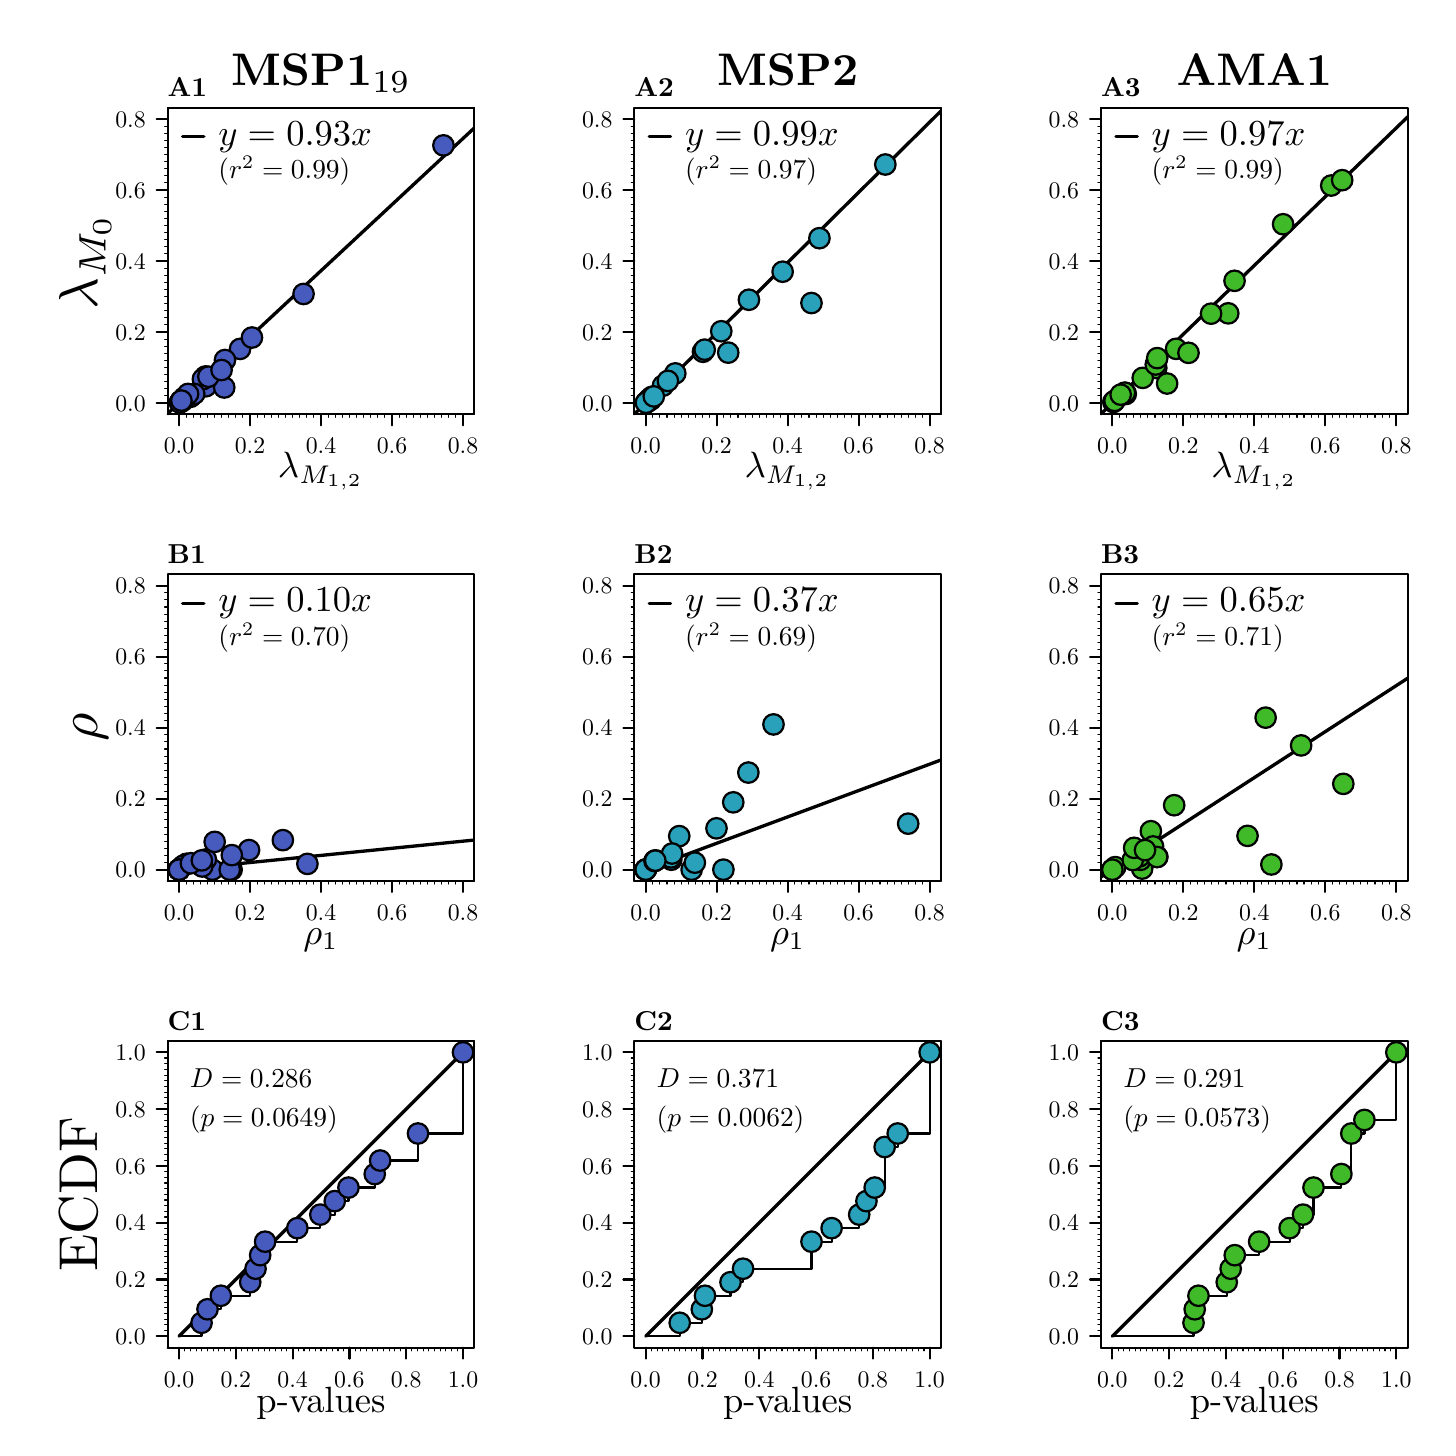
\begin{tikzpicture}[x=1pt,y=1pt]
\definecolor{fillColor}{RGB}{255,255,255}
\path[use as bounding box,fill=fillColor,fill opacity=0.00] (0,0) rectangle (505.89,505.89);
\begin{scope}
\path[clip] (  0.00,  0.00) rectangle (505.89,505.89);
\definecolor{drawColor}{RGB}{0,0,0}

\path[draw=drawColor,line width= 0.4pt,line join=round,line cap=round] ( 50.59,366.17) --
	(161.40,366.17) --
	(161.40,476.98) --
	( 50.59,476.98) --
	( 50.59,366.17);
\end{scope}
\begin{scope}
\path[clip] (  0.00,337.26) rectangle (168.63,505.89);
\definecolor{drawColor}{RGB}{0,0,0}

\node[text=drawColor,anchor=base,inner sep=0pt, outer sep=0pt, scale=  1.65] at (106.00,484.90) {\bfseries MSP1$_{19}$};

\node[text=drawColor,anchor=base west,inner sep=0pt, outer sep=0pt, scale=  0.99] at ( 50.59,480.94) {\bfseries A1};
\end{scope}
\begin{scope}
\path[clip] (  0.00,  0.00) rectangle (505.89,505.89);
\definecolor{drawColor}{RGB}{0,0,0}

\path[draw=drawColor,line width= 0.8pt,line join=round,line cap=round] ( 54.69,366.17) -- (157.30,366.17);

\path[draw=drawColor,line width= 0.8pt,line join=round,line cap=round] ( 54.69,366.17) -- ( 54.69,362.21);

\path[draw=drawColor,line width= 0.8pt,line join=round,line cap=round] ( 80.34,366.17) -- ( 80.34,362.21);

\path[draw=drawColor,line width= 0.8pt,line join=round,line cap=round] (106.00,366.17) -- (106.00,362.21);

\path[draw=drawColor,line width= 0.8pt,line join=round,line cap=round] (131.65,366.17) -- (131.65,362.21);

\path[draw=drawColor,line width= 0.8pt,line join=round,line cap=round] (157.30,366.17) -- (157.30,362.21);

\node[text=drawColor,anchor=base,inner sep=0pt, outer sep=0pt, scale=  0.86] at ( 54.69,351.91) {0.0};

\node[text=drawColor,anchor=base,inner sep=0pt, outer sep=0pt, scale=  0.86] at ( 80.34,351.91) {0.2};

\node[text=drawColor,anchor=base,inner sep=0pt, outer sep=0pt, scale=  0.86] at (106.00,351.91) {0.4};

\node[text=drawColor,anchor=base,inner sep=0pt, outer sep=0pt, scale=  0.86] at (131.65,351.91) {0.6};

\node[text=drawColor,anchor=base,inner sep=0pt, outer sep=0pt, scale=  0.86] at (157.30,351.91) {0.8};

\path[draw=drawColor,line width= 0.4pt,line join=round,line cap=round] ( 54.69,366.17) -- (157.30,366.17);

\path[draw=drawColor,line width= 0.4pt,line join=round,line cap=round] ( 54.69,366.17) -- ( 54.69,365.06);

\path[draw=drawColor,line width= 0.4pt,line join=round,line cap=round] ( 57.26,366.17) -- ( 57.26,365.06);

\path[draw=drawColor,line width= 0.4pt,line join=round,line cap=round] ( 59.82,366.17) -- ( 59.82,365.06);

\path[draw=drawColor,line width= 0.4pt,line join=round,line cap=round] ( 62.39,366.17) -- ( 62.39,365.06);

\path[draw=drawColor,line width= 0.4pt,line join=round,line cap=round] ( 64.95,366.17) -- ( 64.95,365.06);

\path[draw=drawColor,line width= 0.4pt,line join=round,line cap=round] ( 67.52,366.17) -- ( 67.52,365.06);

\path[draw=drawColor,line width= 0.4pt,line join=round,line cap=round] ( 70.08,366.17) -- ( 70.08,365.06);

\path[draw=drawColor,line width= 0.4pt,line join=round,line cap=round] ( 72.65,366.17) -- ( 72.65,365.06);

\path[draw=drawColor,line width= 0.4pt,line join=round,line cap=round] ( 75.21,366.17) -- ( 75.21,365.06);

\path[draw=drawColor,line width= 0.4pt,line join=round,line cap=round] ( 77.78,366.17) -- ( 77.78,365.06);

\path[draw=drawColor,line width= 0.4pt,line join=round,line cap=round] ( 80.34,366.17) -- ( 80.34,365.06);

\path[draw=drawColor,line width= 0.4pt,line join=round,line cap=round] ( 82.91,366.17) -- ( 82.91,365.06);

\path[draw=drawColor,line width= 0.4pt,line join=round,line cap=round] ( 85.47,366.17) -- ( 85.47,365.06);

\path[draw=drawColor,line width= 0.4pt,line join=round,line cap=round] ( 88.04,366.17) -- ( 88.04,365.06);

\path[draw=drawColor,line width= 0.4pt,line join=round,line cap=round] ( 90.61,366.17) -- ( 90.61,365.06);

\path[draw=drawColor,line width= 0.4pt,line join=round,line cap=round] ( 93.17,366.17) -- ( 93.17,365.06);

\path[draw=drawColor,line width= 0.4pt,line join=round,line cap=round] ( 95.74,366.17) -- ( 95.74,365.06);

\path[draw=drawColor,line width= 0.4pt,line join=round,line cap=round] ( 98.30,366.17) -- ( 98.30,365.06);

\path[draw=drawColor,line width= 0.4pt,line join=round,line cap=round] (100.87,366.17) -- (100.87,365.06);

\path[draw=drawColor,line width= 0.4pt,line join=round,line cap=round] (103.43,366.17) -- (103.43,365.06);

\path[draw=drawColor,line width= 0.4pt,line join=round,line cap=round] (106.00,366.17) -- (106.00,365.06);

\path[draw=drawColor,line width= 0.4pt,line join=round,line cap=round] (108.56,366.17) -- (108.56,365.06);

\path[draw=drawColor,line width= 0.4pt,line join=round,line cap=round] (111.13,366.17) -- (111.13,365.06);

\path[draw=drawColor,line width= 0.4pt,line join=round,line cap=round] (113.69,366.17) -- (113.69,365.06);

\path[draw=drawColor,line width= 0.4pt,line join=round,line cap=round] (116.26,366.17) -- (116.26,365.06);

\path[draw=drawColor,line width= 0.4pt,line join=round,line cap=round] (118.82,366.17) -- (118.82,365.06);

\path[draw=drawColor,line width= 0.4pt,line join=round,line cap=round] (121.39,366.17) -- (121.39,365.06);

\path[draw=drawColor,line width= 0.4pt,line join=round,line cap=round] (123.95,366.17) -- (123.95,365.06);

\path[draw=drawColor,line width= 0.4pt,line join=round,line cap=round] (126.52,366.17) -- (126.52,365.06);

\path[draw=drawColor,line width= 0.4pt,line join=round,line cap=round] (129.08,366.17) -- (129.08,365.06);

\path[draw=drawColor,line width= 0.4pt,line join=round,line cap=round] (131.65,366.17) -- (131.65,365.06);

\path[draw=drawColor,line width= 0.4pt,line join=round,line cap=round] (134.21,366.17) -- (134.21,365.06);

\path[draw=drawColor,line width= 0.4pt,line join=round,line cap=round] (136.78,366.17) -- (136.78,365.06);

\path[draw=drawColor,line width= 0.4pt,line join=round,line cap=round] (139.34,366.17) -- (139.34,365.06);

\path[draw=drawColor,line width= 0.4pt,line join=round,line cap=round] (141.91,366.17) -- (141.91,365.06);

\path[draw=drawColor,line width= 0.4pt,line join=round,line cap=round] (144.47,366.17) -- (144.47,365.06);

\path[draw=drawColor,line width= 0.4pt,line join=round,line cap=round] (147.04,366.17) -- (147.04,365.06);

\path[draw=drawColor,line width= 0.4pt,line join=round,line cap=round] (149.60,366.17) -- (149.60,365.06);

\path[draw=drawColor,line width= 0.4pt,line join=round,line cap=round] (152.17,366.17) -- (152.17,365.06);

\path[draw=drawColor,line width= 0.4pt,line join=round,line cap=round] (154.73,366.17) -- (154.73,365.06);

\path[draw=drawColor,line width= 0.4pt,line join=round,line cap=round] (157.30,366.17) -- (157.30,365.06);

\path[draw=drawColor,line width= 0.8pt,line join=round,line cap=round] ( 50.59,370.27) -- ( 50.59,472.88);

\path[draw=drawColor,line width= 0.8pt,line join=round,line cap=round] ( 50.59,370.27) -- ( 46.63,370.27);

\path[draw=drawColor,line width= 0.8pt,line join=round,line cap=round] ( 50.59,395.92) -- ( 46.63,395.92);

\path[draw=drawColor,line width= 0.8pt,line join=round,line cap=round] ( 50.59,421.58) -- ( 46.63,421.58);

\path[draw=drawColor,line width= 0.8pt,line join=round,line cap=round] ( 50.59,447.23) -- ( 46.63,447.23);

\path[draw=drawColor,line width= 0.8pt,line join=round,line cap=round] ( 50.59,472.88) -- ( 46.63,472.88);

\node[text=drawColor,anchor=base east,inner sep=0pt, outer sep=0pt, scale=  0.86] at ( 42.67,367.32) {0.0};

\node[text=drawColor,anchor=base east,inner sep=0pt, outer sep=0pt, scale=  0.86] at ( 42.67,392.97) {0.2};

\node[text=drawColor,anchor=base east,inner sep=0pt, outer sep=0pt, scale=  0.86] at ( 42.67,418.62) {0.4};

\node[text=drawColor,anchor=base east,inner sep=0pt, outer sep=0pt, scale=  0.86] at ( 42.67,444.27) {0.6};

\node[text=drawColor,anchor=base east,inner sep=0pt, outer sep=0pt, scale=  0.86] at ( 42.67,469.92) {0.8};

\path[draw=drawColor,line width= 0.4pt,line join=round,line cap=round] ( 50.59,370.27) -- ( 50.59,472.88);

\path[draw=drawColor,line width= 0.4pt,line join=round,line cap=round] ( 50.59,370.27) -- ( 49.48,370.27);

\path[draw=drawColor,line width= 0.4pt,line join=round,line cap=round] ( 50.59,372.84) -- ( 49.48,372.84);

\path[draw=drawColor,line width= 0.4pt,line join=round,line cap=round] ( 50.59,375.40) -- ( 49.48,375.40);

\path[draw=drawColor,line width= 0.4pt,line join=round,line cap=round] ( 50.59,377.97) -- ( 49.48,377.97);

\path[draw=drawColor,line width= 0.4pt,line join=round,line cap=round] ( 50.59,380.53) -- ( 49.48,380.53);

\path[draw=drawColor,line width= 0.4pt,line join=round,line cap=round] ( 50.59,383.10) -- ( 49.48,383.10);

\path[draw=drawColor,line width= 0.4pt,line join=round,line cap=round] ( 50.59,385.66) -- ( 49.48,385.66);

\path[draw=drawColor,line width= 0.4pt,line join=round,line cap=round] ( 50.59,388.23) -- ( 49.48,388.23);

\path[draw=drawColor,line width= 0.4pt,line join=round,line cap=round] ( 50.59,390.79) -- ( 49.48,390.79);

\path[draw=drawColor,line width= 0.4pt,line join=round,line cap=round] ( 50.59,393.36) -- ( 49.48,393.36);

\path[draw=drawColor,line width= 0.4pt,line join=round,line cap=round] ( 50.59,395.92) -- ( 49.48,395.92);

\path[draw=drawColor,line width= 0.4pt,line join=round,line cap=round] ( 50.59,398.49) -- ( 49.48,398.49);

\path[draw=drawColor,line width= 0.4pt,line join=round,line cap=round] ( 50.59,401.05) -- ( 49.48,401.05);

\path[draw=drawColor,line width= 0.4pt,line join=round,line cap=round] ( 50.59,403.62) -- ( 49.48,403.62);

\path[draw=drawColor,line width= 0.4pt,line join=round,line cap=round] ( 50.59,406.18) -- ( 49.48,406.18);

\path[draw=drawColor,line width= 0.4pt,line join=round,line cap=round] ( 50.59,408.75) -- ( 49.48,408.75);

\path[draw=drawColor,line width= 0.4pt,line join=round,line cap=round] ( 50.59,411.31) -- ( 49.48,411.31);

\path[draw=drawColor,line width= 0.4pt,line join=round,line cap=round] ( 50.59,413.88) -- ( 49.48,413.88);

\path[draw=drawColor,line width= 0.4pt,line join=round,line cap=round] ( 50.59,416.44) -- ( 49.48,416.44);

\path[draw=drawColor,line width= 0.4pt,line join=round,line cap=round] ( 50.59,419.01) -- ( 49.48,419.01);

\path[draw=drawColor,line width= 0.4pt,line join=round,line cap=round] ( 50.59,421.58) -- ( 49.48,421.58);

\path[draw=drawColor,line width= 0.4pt,line join=round,line cap=round] ( 50.59,424.14) -- ( 49.48,424.14);

\path[draw=drawColor,line width= 0.4pt,line join=round,line cap=round] ( 50.59,426.71) -- ( 49.48,426.71);

\path[draw=drawColor,line width= 0.4pt,line join=round,line cap=round] ( 50.59,429.27) -- ( 49.48,429.27);

\path[draw=drawColor,line width= 0.4pt,line join=round,line cap=round] ( 50.59,431.84) -- ( 49.48,431.84);

\path[draw=drawColor,line width= 0.4pt,line join=round,line cap=round] ( 50.59,434.40) -- ( 49.48,434.40);

\path[draw=drawColor,line width= 0.4pt,line join=round,line cap=round] ( 50.59,436.97) -- ( 49.48,436.97);

\path[draw=drawColor,line width= 0.4pt,line join=round,line cap=round] ( 50.59,439.53) -- ( 49.48,439.53);

\path[draw=drawColor,line width= 0.4pt,line join=round,line cap=round] ( 50.59,442.10) -- ( 49.48,442.10);

\path[draw=drawColor,line width= 0.4pt,line join=round,line cap=round] ( 50.59,444.66) -- ( 49.48,444.66);

\path[draw=drawColor,line width= 0.4pt,line join=round,line cap=round] ( 50.59,447.23) -- ( 49.48,447.23);

\path[draw=drawColor,line width= 0.4pt,line join=round,line cap=round] ( 50.59,449.79) -- ( 49.48,449.79);

\path[draw=drawColor,line width= 0.4pt,line join=round,line cap=round] ( 50.59,452.36) -- ( 49.48,452.36);

\path[draw=drawColor,line width= 0.4pt,line join=round,line cap=round] ( 50.59,454.92) -- ( 49.48,454.92);

\path[draw=drawColor,line width= 0.4pt,line join=round,line cap=round] ( 50.59,457.49) -- ( 49.48,457.49);

\path[draw=drawColor,line width= 0.4pt,line join=round,line cap=round] ( 50.59,460.05) -- ( 49.48,460.05);

\path[draw=drawColor,line width= 0.4pt,line join=round,line cap=round] ( 50.59,462.62) -- ( 49.48,462.62);

\path[draw=drawColor,line width= 0.4pt,line join=round,line cap=round] ( 50.59,465.18) -- ( 49.48,465.18);

\path[draw=drawColor,line width= 0.4pt,line join=round,line cap=round] ( 50.59,467.75) -- ( 49.48,467.75);

\path[draw=drawColor,line width= 0.4pt,line join=round,line cap=round] ( 50.59,470.31) -- ( 49.48,470.31);

\path[draw=drawColor,line width= 0.4pt,line join=round,line cap=round] ( 50.59,472.88) -- ( 49.48,472.88);
\end{scope}
\begin{scope}
\path[clip] (  0.00,337.26) rectangle (168.63,505.89);
\definecolor{drawColor}{RGB}{0,0,0}

\node[text=drawColor,rotate= 90.00,anchor=base,inner sep=0pt, outer sep=0pt, scale=  1.98] at ( 25.24,421.58) {$\lambda_{M_0}$};

\node[text=drawColor,anchor=base west,inner sep=0pt, outer sep=0pt, scale=  1.32] at ( 90.45,343.33) {$\lambda_{M_{1,2}}$};
\end{scope}
\begin{scope}
\path[clip] ( 50.59,366.17) rectangle (161.40,476.98);
\definecolor{drawColor}{RGB}{0,0,0}

\path[draw=drawColor,line width= 1.2pt,line join=round,line cap=round] ( 50.59,366.45) -- (161.40,469.66);
\definecolor{fillColor}{RGB}{71,91,191}

\path[draw=drawColor,line width= 0.8pt,line join=round,line cap=round,fill=fillColor] ( 56.59,372.12) circle (  3.71);

\path[draw=drawColor,line width= 0.8pt,line join=round,line cap=round,fill=fillColor] ( 64.39,376.31) circle (  3.71);

\path[draw=drawColor,line width= 0.8pt,line join=round,line cap=round,fill=fillColor] ( 58.87,372.50) circle (  3.71);

\path[draw=drawColor,line width= 0.8pt,line join=round,line cap=round,fill=fillColor] ( 99.69,409.66) circle (  3.71);

\path[draw=drawColor,line width= 0.8pt,line join=round,line cap=round,fill=fillColor] ( 55.39,370.96) circle (  3.71);

\path[draw=drawColor,line width= 0.8pt,line join=round,line cap=round,fill=fillColor] ( 56.67,372.23) circle (  3.71);

\path[draw=drawColor,line width= 0.8pt,line join=round,line cap=round,fill=fillColor] ( 64.26,379.84) circle (  3.71);

\path[draw=drawColor,line width= 0.8pt,line join=round,line cap=round,fill=fillColor] ( 63.32,378.88) circle (  3.71);

\path[draw=drawColor,line width= 0.8pt,line join=round,line cap=round,fill=fillColor] ( 55.89,370.96) circle (  3.71);

\path[draw=drawColor,line width= 0.8pt,line join=round,line cap=round,fill=fillColor] ( 55.28,370.86) circle (  3.71);

\path[draw=drawColor,line width= 0.8pt,line join=round,line cap=round,fill=fillColor] ( 60.17,373.54) circle (  3.71);

\path[draw=drawColor,line width= 0.8pt,line join=round,line cap=round,fill=fillColor] ( 76.75,389.81) circle (  3.71);

\path[draw=drawColor,line width= 0.8pt,line join=round,line cap=round,fill=fillColor] ( 55.00,370.41) circle (  3.71);

\path[draw=drawColor,line width= 0.8pt,line join=round,line cap=round,fill=fillColor] ( 71.03,375.86) circle (  3.71);

\path[draw=drawColor,line width= 0.8pt,line join=round,line cap=round,fill=fillColor] ( 57.96,373.54) circle (  3.71);

\path[draw=drawColor,line width= 0.8pt,line join=round,line cap=round,fill=fillColor] ( 65.30,379.76) circle (  3.71);

\path[draw=drawColor,line width= 0.8pt,line join=round,line cap=round,fill=fillColor] ( 55.55,371.13) circle (  3.71);

\path[draw=drawColor,line width= 0.8pt,line join=round,line cap=round,fill=fillColor] ( 71.30,385.79) circle (  3.71);

\path[draw=drawColor,line width= 0.8pt,line join=round,line cap=round,fill=fillColor] ( 70.06,382.17) circle (  3.71);

\path[draw=drawColor,line width= 0.8pt,line join=round,line cap=round,fill=fillColor] ( 81.04,393.92) circle (  3.71);

\path[draw=drawColor,line width= 0.8pt,line join=round,line cap=round,fill=fillColor] (150.24,463.36) circle (  3.71);

\path[draw=drawColor,line width= 1.2pt,line join=round,line cap=round] ( 55.98,466.46) -- ( 63.67,466.46);

\node[text=drawColor,anchor=base west,inner sep=0pt, outer sep=0pt, scale=  1.32] at ( 68.91,463.43) {$y=0.93x$};

\node[text=drawColor,anchor=base west,inner sep=0pt, outer sep=0pt, scale=  0.99] at ( 68.91,451.37) {$(r^2=0.99)$};
\end{scope}
\begin{scope}
\path[clip] (  0.00,  0.00) rectangle (505.89,505.89);
\definecolor{drawColor}{RGB}{0,0,0}

\path[draw=drawColor,line width= 0.8pt,line join=round,line cap=round] ( 50.59,366.17) --
	(161.40,366.17) --
	(161.40,476.98) --
	( 50.59,476.98) --
	( 50.59,366.17);
\end{scope}
\begin{scope}
\path[clip] (  0.00,  0.00) rectangle (505.89,505.89);
\definecolor{drawColor}{RGB}{0,0,0}

\path[draw=drawColor,line width= 0.4pt,line join=round,line cap=round] (219.22,366.17) --
	(330.03,366.17) --
	(330.03,476.98) --
	(219.22,476.98) --
	(219.22,366.17);
\end{scope}
\begin{scope}
\path[clip] (168.63,337.26) rectangle (337.26,505.89);
\definecolor{drawColor}{RGB}{0,0,0}

\node[text=drawColor,anchor=base,inner sep=0pt, outer sep=0pt, scale=  1.65] at (274.63,484.90) {\bfseries MSP2};

\node[text=drawColor,anchor=base west,inner sep=0pt, outer sep=0pt, scale=  0.99] at (219.22,480.94) {\bfseries A2};
\end{scope}
\begin{scope}
\path[clip] (  0.00,  0.00) rectangle (505.89,505.89);
\definecolor{drawColor}{RGB}{0,0,0}

\path[draw=drawColor,line width= 0.8pt,line join=round,line cap=round] (223.32,366.17) -- (325.93,366.17);

\path[draw=drawColor,line width= 0.8pt,line join=round,line cap=round] (223.32,366.17) -- (223.32,362.21);

\path[draw=drawColor,line width= 0.8pt,line join=round,line cap=round] (248.97,366.17) -- (248.97,362.21);

\path[draw=drawColor,line width= 0.8pt,line join=round,line cap=round] (274.63,366.17) -- (274.63,362.21);

\path[draw=drawColor,line width= 0.8pt,line join=round,line cap=round] (300.28,366.17) -- (300.28,362.21);

\path[draw=drawColor,line width= 0.8pt,line join=round,line cap=round] (325.93,366.17) -- (325.93,362.21);

\node[text=drawColor,anchor=base,inner sep=0pt, outer sep=0pt, scale=  0.86] at (223.32,351.91) {0.0};

\node[text=drawColor,anchor=base,inner sep=0pt, outer sep=0pt, scale=  0.86] at (248.97,351.91) {0.2};

\node[text=drawColor,anchor=base,inner sep=0pt, outer sep=0pt, scale=  0.86] at (274.63,351.91) {0.4};

\node[text=drawColor,anchor=base,inner sep=0pt, outer sep=0pt, scale=  0.86] at (300.28,351.91) {0.6};

\node[text=drawColor,anchor=base,inner sep=0pt, outer sep=0pt, scale=  0.86] at (325.93,351.91) {0.8};

\path[draw=drawColor,line width= 0.4pt,line join=round,line cap=round] (223.32,366.17) -- (325.93,366.17);

\path[draw=drawColor,line width= 0.4pt,line join=round,line cap=round] (223.32,366.17) -- (223.32,365.06);

\path[draw=drawColor,line width= 0.4pt,line join=round,line cap=round] (225.89,366.17) -- (225.89,365.06);

\path[draw=drawColor,line width= 0.4pt,line join=round,line cap=round] (228.45,366.17) -- (228.45,365.06);

\path[draw=drawColor,line width= 0.4pt,line join=round,line cap=round] (231.02,366.17) -- (231.02,365.06);

\path[draw=drawColor,line width= 0.4pt,line join=round,line cap=round] (233.58,366.17) -- (233.58,365.06);

\path[draw=drawColor,line width= 0.4pt,line join=round,line cap=round] (236.15,366.17) -- (236.15,365.06);

\path[draw=drawColor,line width= 0.4pt,line join=round,line cap=round] (238.71,366.17) -- (238.71,365.06);

\path[draw=drawColor,line width= 0.4pt,line join=round,line cap=round] (241.28,366.17) -- (241.28,365.06);

\path[draw=drawColor,line width= 0.4pt,line join=round,line cap=round] (243.84,366.17) -- (243.84,365.06);

\path[draw=drawColor,line width= 0.4pt,line join=round,line cap=round] (246.41,366.17) -- (246.41,365.06);

\path[draw=drawColor,line width= 0.4pt,line join=round,line cap=round] (248.97,366.17) -- (248.97,365.06);

\path[draw=drawColor,line width= 0.4pt,line join=round,line cap=round] (251.54,366.17) -- (251.54,365.06);

\path[draw=drawColor,line width= 0.4pt,line join=round,line cap=round] (254.10,366.17) -- (254.10,365.06);

\path[draw=drawColor,line width= 0.4pt,line join=round,line cap=round] (256.67,366.17) -- (256.67,365.06);

\path[draw=drawColor,line width= 0.4pt,line join=round,line cap=round] (259.24,366.17) -- (259.24,365.06);

\path[draw=drawColor,line width= 0.4pt,line join=round,line cap=round] (261.80,366.17) -- (261.80,365.06);

\path[draw=drawColor,line width= 0.4pt,line join=round,line cap=round] (264.37,366.17) -- (264.37,365.06);

\path[draw=drawColor,line width= 0.4pt,line join=round,line cap=round] (266.93,366.17) -- (266.93,365.06);

\path[draw=drawColor,line width= 0.4pt,line join=round,line cap=round] (269.50,366.17) -- (269.50,365.06);

\path[draw=drawColor,line width= 0.4pt,line join=round,line cap=round] (272.06,366.17) -- (272.06,365.06);

\path[draw=drawColor,line width= 0.4pt,line join=round,line cap=round] (274.63,366.17) -- (274.63,365.06);

\path[draw=drawColor,line width= 0.4pt,line join=round,line cap=round] (277.19,366.17) -- (277.19,365.06);

\path[draw=drawColor,line width= 0.4pt,line join=round,line cap=round] (279.76,366.17) -- (279.76,365.06);

\path[draw=drawColor,line width= 0.4pt,line join=round,line cap=round] (282.32,366.17) -- (282.32,365.06);

\path[draw=drawColor,line width= 0.4pt,line join=round,line cap=round] (284.89,366.17) -- (284.89,365.06);

\path[draw=drawColor,line width= 0.4pt,line join=round,line cap=round] (287.45,366.17) -- (287.45,365.06);

\path[draw=drawColor,line width= 0.4pt,line join=round,line cap=round] (290.02,366.17) -- (290.02,365.06);

\path[draw=drawColor,line width= 0.4pt,line join=round,line cap=round] (292.58,366.17) -- (292.58,365.06);

\path[draw=drawColor,line width= 0.4pt,line join=round,line cap=round] (295.15,366.17) -- (295.15,365.06);

\path[draw=drawColor,line width= 0.4pt,line join=round,line cap=round] (297.71,366.17) -- (297.71,365.06);

\path[draw=drawColor,line width= 0.4pt,line join=round,line cap=round] (300.28,366.17) -- (300.28,365.06);

\path[draw=drawColor,line width= 0.4pt,line join=round,line cap=round] (302.84,366.17) -- (302.84,365.06);

\path[draw=drawColor,line width= 0.4pt,line join=round,line cap=round] (305.41,366.17) -- (305.41,365.06);

\path[draw=drawColor,line width= 0.4pt,line join=round,line cap=round] (307.97,366.17) -- (307.97,365.06);

\path[draw=drawColor,line width= 0.4pt,line join=round,line cap=round] (310.54,366.17) -- (310.54,365.06);

\path[draw=drawColor,line width= 0.4pt,line join=round,line cap=round] (313.10,366.17) -- (313.10,365.06);

\path[draw=drawColor,line width= 0.4pt,line join=round,line cap=round] (315.67,366.17) -- (315.67,365.06);

\path[draw=drawColor,line width= 0.4pt,line join=round,line cap=round] (318.23,366.17) -- (318.23,365.06);

\path[draw=drawColor,line width= 0.4pt,line join=round,line cap=round] (320.80,366.17) -- (320.80,365.06);

\path[draw=drawColor,line width= 0.4pt,line join=round,line cap=round] (323.36,366.17) -- (323.36,365.06);

\path[draw=drawColor,line width= 0.4pt,line join=round,line cap=round] (325.93,366.17) -- (325.93,365.06);

\path[draw=drawColor,line width= 0.8pt,line join=round,line cap=round] (219.22,370.27) -- (219.22,472.88);

\path[draw=drawColor,line width= 0.8pt,line join=round,line cap=round] (219.22,370.27) -- (215.26,370.27);

\path[draw=drawColor,line width= 0.8pt,line join=round,line cap=round] (219.22,395.92) -- (215.26,395.92);

\path[draw=drawColor,line width= 0.8pt,line join=round,line cap=round] (219.22,421.58) -- (215.26,421.58);

\path[draw=drawColor,line width= 0.8pt,line join=round,line cap=round] (219.22,447.23) -- (215.26,447.23);

\path[draw=drawColor,line width= 0.8pt,line join=round,line cap=round] (219.22,472.88) -- (215.26,472.88);

\node[text=drawColor,anchor=base east,inner sep=0pt, outer sep=0pt, scale=  0.86] at (211.30,367.32) {0.0};

\node[text=drawColor,anchor=base east,inner sep=0pt, outer sep=0pt, scale=  0.86] at (211.30,392.97) {0.2};

\node[text=drawColor,anchor=base east,inner sep=0pt, outer sep=0pt, scale=  0.86] at (211.30,418.62) {0.4};

\node[text=drawColor,anchor=base east,inner sep=0pt, outer sep=0pt, scale=  0.86] at (211.30,444.27) {0.6};

\node[text=drawColor,anchor=base east,inner sep=0pt, outer sep=0pt, scale=  0.86] at (211.30,469.92) {0.8};

\path[draw=drawColor,line width= 0.4pt,line join=round,line cap=round] (219.22,370.27) -- (219.22,472.88);

\path[draw=drawColor,line width= 0.4pt,line join=round,line cap=round] (219.22,370.27) -- (218.11,370.27);

\path[draw=drawColor,line width= 0.4pt,line join=round,line cap=round] (219.22,372.84) -- (218.11,372.84);

\path[draw=drawColor,line width= 0.4pt,line join=round,line cap=round] (219.22,375.40) -- (218.11,375.40);

\path[draw=drawColor,line width= 0.4pt,line join=round,line cap=round] (219.22,377.97) -- (218.11,377.97);

\path[draw=drawColor,line width= 0.4pt,line join=round,line cap=round] (219.22,380.53) -- (218.11,380.53);

\path[draw=drawColor,line width= 0.4pt,line join=round,line cap=round] (219.22,383.10) -- (218.11,383.10);

\path[draw=drawColor,line width= 0.4pt,line join=round,line cap=round] (219.22,385.66) -- (218.11,385.66);

\path[draw=drawColor,line width= 0.4pt,line join=round,line cap=round] (219.22,388.23) -- (218.11,388.23);

\path[draw=drawColor,line width= 0.4pt,line join=round,line cap=round] (219.22,390.79) -- (218.11,390.79);

\path[draw=drawColor,line width= 0.4pt,line join=round,line cap=round] (219.22,393.36) -- (218.11,393.36);

\path[draw=drawColor,line width= 0.4pt,line join=round,line cap=round] (219.22,395.92) -- (218.11,395.92);

\path[draw=drawColor,line width= 0.4pt,line join=round,line cap=round] (219.22,398.49) -- (218.11,398.49);

\path[draw=drawColor,line width= 0.4pt,line join=round,line cap=round] (219.22,401.05) -- (218.11,401.05);

\path[draw=drawColor,line width= 0.4pt,line join=round,line cap=round] (219.22,403.62) -- (218.11,403.62);

\path[draw=drawColor,line width= 0.4pt,line join=round,line cap=round] (219.22,406.18) -- (218.11,406.18);

\path[draw=drawColor,line width= 0.4pt,line join=round,line cap=round] (219.22,408.75) -- (218.11,408.75);

\path[draw=drawColor,line width= 0.4pt,line join=round,line cap=round] (219.22,411.31) -- (218.11,411.31);

\path[draw=drawColor,line width= 0.4pt,line join=round,line cap=round] (219.22,413.88) -- (218.11,413.88);

\path[draw=drawColor,line width= 0.4pt,line join=round,line cap=round] (219.22,416.44) -- (218.11,416.44);

\path[draw=drawColor,line width= 0.4pt,line join=round,line cap=round] (219.22,419.01) -- (218.11,419.01);

\path[draw=drawColor,line width= 0.4pt,line join=round,line cap=round] (219.22,421.58) -- (218.11,421.58);

\path[draw=drawColor,line width= 0.4pt,line join=round,line cap=round] (219.22,424.14) -- (218.11,424.14);

\path[draw=drawColor,line width= 0.4pt,line join=round,line cap=round] (219.22,426.71) -- (218.11,426.71);

\path[draw=drawColor,line width= 0.4pt,line join=round,line cap=round] (219.22,429.27) -- (218.11,429.27);

\path[draw=drawColor,line width= 0.4pt,line join=round,line cap=round] (219.22,431.84) -- (218.11,431.84);

\path[draw=drawColor,line width= 0.4pt,line join=round,line cap=round] (219.22,434.40) -- (218.11,434.40);

\path[draw=drawColor,line width= 0.4pt,line join=round,line cap=round] (219.22,436.97) -- (218.11,436.97);

\path[draw=drawColor,line width= 0.4pt,line join=round,line cap=round] (219.22,439.53) -- (218.11,439.53);

\path[draw=drawColor,line width= 0.4pt,line join=round,line cap=round] (219.22,442.10) -- (218.11,442.10);

\path[draw=drawColor,line width= 0.4pt,line join=round,line cap=round] (219.22,444.66) -- (218.11,444.66);

\path[draw=drawColor,line width= 0.4pt,line join=round,line cap=round] (219.22,447.23) -- (218.11,447.23);

\path[draw=drawColor,line width= 0.4pt,line join=round,line cap=round] (219.22,449.79) -- (218.11,449.79);

\path[draw=drawColor,line width= 0.4pt,line join=round,line cap=round] (219.22,452.36) -- (218.11,452.36);

\path[draw=drawColor,line width= 0.4pt,line join=round,line cap=round] (219.22,454.92) -- (218.11,454.92);

\path[draw=drawColor,line width= 0.4pt,line join=round,line cap=round] (219.22,457.49) -- (218.11,457.49);

\path[draw=drawColor,line width= 0.4pt,line join=round,line cap=round] (219.22,460.05) -- (218.11,460.05);

\path[draw=drawColor,line width= 0.4pt,line join=round,line cap=round] (219.22,462.62) -- (218.11,462.62);

\path[draw=drawColor,line width= 0.4pt,line join=round,line cap=round] (219.22,465.18) -- (218.11,465.18);

\path[draw=drawColor,line width= 0.4pt,line join=round,line cap=round] (219.22,467.75) -- (218.11,467.75);

\path[draw=drawColor,line width= 0.4pt,line join=round,line cap=round] (219.22,470.31) -- (218.11,470.31);

\path[draw=drawColor,line width= 0.4pt,line join=round,line cap=round] (219.22,472.88) -- (218.11,472.88);
\end{scope}
\begin{scope}
\path[clip] (168.63,337.26) rectangle (337.26,505.89);
\definecolor{drawColor}{RGB}{0,0,0}

\node[text=drawColor,anchor=base west,inner sep=0pt, outer sep=0pt, scale=  1.32] at (259.08,343.33) {$\lambda_{M_{1,2}}$};
\end{scope}
\begin{scope}
\path[clip] (219.22,366.17) rectangle (330.03,476.98);
\definecolor{drawColor}{RGB}{0,0,0}

\path[draw=drawColor,line width= 1.2pt,line join=round,line cap=round] (219.22,366.21) -- (330.03,475.80);
\definecolor{fillColor}{RGB}{42,161,186}

\path[draw=drawColor,line width= 0.8pt,line join=round,line cap=round,fill=fillColor] (223.75,370.54) circle (  3.71);

\path[draw=drawColor,line width= 0.8pt,line join=round,line cap=round,fill=fillColor] (224.66,371.64) circle (  3.71);

\path[draw=drawColor,line width= 0.8pt,line join=round,line cap=round,fill=fillColor] (223.49,370.44) circle (  3.71);

\path[draw=drawColor,line width= 0.8pt,line join=round,line cap=round,fill=fillColor] (225.16,371.44) circle (  3.71);

\path[draw=drawColor,line width= 0.8pt,line join=round,line cap=round,fill=fillColor] (224.26,371.20) circle (  3.71);

\path[draw=drawColor,line width= 0.8pt,line join=round,line cap=round,fill=fillColor] (225.49,372.44) circle (  3.71);

\path[draw=drawColor,line width= 0.8pt,line join=round,line cap=round,fill=fillColor] (260.62,407.57) circle (  3.71);

\path[draw=drawColor,line width= 0.8pt,line join=round,line cap=round,fill=fillColor] (332.78,496.82) circle (  3.71);

\path[draw=drawColor,line width= 0.8pt,line join=round,line cap=round,fill=fillColor] (229.57,376.52) circle (  3.71);

\path[draw=drawColor,line width= 0.8pt,line join=round,line cap=round,fill=fillColor] (250.63,396.19) circle (  3.71);

\path[draw=drawColor,line width= 0.8pt,line join=round,line cap=round,fill=fillColor] (283.22,406.38) circle (  3.71);

\path[draw=drawColor,line width= 0.8pt,line join=round,line cap=round,fill=fillColor] (253.14,388.46) circle (  3.71);

\path[draw=drawColor,line width= 0.8pt,line join=round,line cap=round,fill=fillColor] (223.41,370.36) circle (  3.71);

\path[draw=drawColor,line width= 0.8pt,line join=round,line cap=round,fill=fillColor] (234.01,380.96) circle (  3.71);

\path[draw=drawColor,line width= 0.8pt,line join=round,line cap=round,fill=fillColor] (231.33,378.25) circle (  3.71);

\path[draw=drawColor,line width= 0.8pt,line join=round,line cap=round,fill=fillColor] (272.80,417.70) circle (  3.71);

\path[draw=drawColor,line width= 0.8pt,line join=round,line cap=round,fill=fillColor] (226.25,372.64) circle (  3.71);

\path[draw=drawColor,line width= 0.8pt,line join=round,line cap=round,fill=fillColor] (244.02,388.77) circle (  3.71);

\path[draw=drawColor,line width= 0.8pt,line join=round,line cap=round,fill=fillColor] (244.65,389.54) circle (  3.71);

\path[draw=drawColor,line width= 0.8pt,line join=round,line cap=round,fill=fillColor] (286.10,429.82) circle (  3.71);

\path[draw=drawColor,line width= 0.8pt,line join=round,line cap=round,fill=fillColor] (309.91,456.44) circle (  3.71);

\path[draw=drawColor,line width= 1.2pt,line join=round,line cap=round] (224.61,466.46) -- (232.30,466.46);

\node[text=drawColor,anchor=base west,inner sep=0pt, outer sep=0pt, scale=  1.32] at (237.54,463.43) {$y=0.99x$};

\node[text=drawColor,anchor=base west,inner sep=0pt, outer sep=0pt, scale=  0.99] at (237.54,451.37) {$(r^2=0.97)$};
\end{scope}
\begin{scope}
\path[clip] (  0.00,  0.00) rectangle (505.89,505.89);
\definecolor{drawColor}{RGB}{0,0,0}

\path[draw=drawColor,line width= 0.8pt,line join=round,line cap=round] (219.22,366.17) --
	(330.03,366.17) --
	(330.03,476.98) --
	(219.22,476.98) --
	(219.22,366.17);
\end{scope}
\begin{scope}
\path[clip] (  0.00,  0.00) rectangle (505.89,505.89);
\definecolor{drawColor}{RGB}{0,0,0}

\path[draw=drawColor,line width= 0.4pt,line join=round,line cap=round] (387.85,366.17) --
	(498.66,366.17) --
	(498.66,476.98) --
	(387.85,476.98) --
	(387.85,366.17);
\end{scope}
\begin{scope}
\path[clip] (337.26,337.26) rectangle (505.89,505.89);
\definecolor{drawColor}{RGB}{0,0,0}

\node[text=drawColor,anchor=base west,inner sep=0pt, outer sep=0pt, scale=  0.99] at (387.85,480.94) {\bfseries A3};

\node[text=drawColor,anchor=base,inner sep=0pt, outer sep=0pt, scale=  1.65] at (443.26,484.90) {\bfseries AMA1};
\end{scope}
\begin{scope}
\path[clip] (  0.00,  0.00) rectangle (505.89,505.89);
\definecolor{drawColor}{RGB}{0,0,0}

\path[draw=drawColor,line width= 0.8pt,line join=round,line cap=round] (391.95,366.17) -- (494.56,366.17);

\path[draw=drawColor,line width= 0.8pt,line join=round,line cap=round] (391.95,366.17) -- (391.95,362.21);

\path[draw=drawColor,line width= 0.8pt,line join=round,line cap=round] (417.60,366.17) -- (417.60,362.21);

\path[draw=drawColor,line width= 0.8pt,line join=round,line cap=round] (443.26,366.17) -- (443.26,362.21);

\path[draw=drawColor,line width= 0.8pt,line join=round,line cap=round] (468.91,366.17) -- (468.91,362.21);

\path[draw=drawColor,line width= 0.8pt,line join=round,line cap=round] (494.56,366.17) -- (494.56,362.21);

\node[text=drawColor,anchor=base,inner sep=0pt, outer sep=0pt, scale=  0.86] at (391.95,351.91) {0.0};

\node[text=drawColor,anchor=base,inner sep=0pt, outer sep=0pt, scale=  0.86] at (417.60,351.91) {0.2};

\node[text=drawColor,anchor=base,inner sep=0pt, outer sep=0pt, scale=  0.86] at (443.26,351.91) {0.4};

\node[text=drawColor,anchor=base,inner sep=0pt, outer sep=0pt, scale=  0.86] at (468.91,351.91) {0.6};

\node[text=drawColor,anchor=base,inner sep=0pt, outer sep=0pt, scale=  0.86] at (494.56,351.91) {0.8};

\path[draw=drawColor,line width= 0.4pt,line join=round,line cap=round] (391.95,366.17) -- (494.56,366.17);

\path[draw=drawColor,line width= 0.4pt,line join=round,line cap=round] (391.95,366.17) -- (391.95,365.06);

\path[draw=drawColor,line width= 0.4pt,line join=round,line cap=round] (394.52,366.17) -- (394.52,365.06);

\path[draw=drawColor,line width= 0.4pt,line join=round,line cap=round] (397.08,366.17) -- (397.08,365.06);

\path[draw=drawColor,line width= 0.4pt,line join=round,line cap=round] (399.65,366.17) -- (399.65,365.06);

\path[draw=drawColor,line width= 0.4pt,line join=round,line cap=round] (402.21,366.17) -- (402.21,365.06);

\path[draw=drawColor,line width= 0.4pt,line join=round,line cap=round] (404.78,366.17) -- (404.78,365.06);

\path[draw=drawColor,line width= 0.4pt,line join=round,line cap=round] (407.34,366.17) -- (407.34,365.06);

\path[draw=drawColor,line width= 0.4pt,line join=round,line cap=round] (409.91,366.17) -- (409.91,365.06);

\path[draw=drawColor,line width= 0.4pt,line join=round,line cap=round] (412.47,366.17) -- (412.47,365.06);

\path[draw=drawColor,line width= 0.4pt,line join=round,line cap=round] (415.04,366.17) -- (415.04,365.06);

\path[draw=drawColor,line width= 0.4pt,line join=round,line cap=round] (417.60,366.17) -- (417.60,365.06);

\path[draw=drawColor,line width= 0.4pt,line join=round,line cap=round] (420.17,366.17) -- (420.17,365.06);

\path[draw=drawColor,line width= 0.4pt,line join=round,line cap=round] (422.73,366.17) -- (422.73,365.06);

\path[draw=drawColor,line width= 0.4pt,line join=round,line cap=round] (425.30,366.17) -- (425.30,365.06);

\path[draw=drawColor,line width= 0.4pt,line join=round,line cap=round] (427.87,366.17) -- (427.87,365.06);

\path[draw=drawColor,line width= 0.4pt,line join=round,line cap=round] (430.43,366.17) -- (430.43,365.06);

\path[draw=drawColor,line width= 0.4pt,line join=round,line cap=round] (433.00,366.17) -- (433.00,365.06);

\path[draw=drawColor,line width= 0.4pt,line join=round,line cap=round] (435.56,366.17) -- (435.56,365.06);

\path[draw=drawColor,line width= 0.4pt,line join=round,line cap=round] (438.13,366.17) -- (438.13,365.06);

\path[draw=drawColor,line width= 0.4pt,line join=round,line cap=round] (440.69,366.17) -- (440.69,365.06);

\path[draw=drawColor,line width= 0.4pt,line join=round,line cap=round] (443.26,366.17) -- (443.26,365.06);

\path[draw=drawColor,line width= 0.4pt,line join=round,line cap=round] (445.82,366.17) -- (445.82,365.06);

\path[draw=drawColor,line width= 0.4pt,line join=round,line cap=round] (448.39,366.17) -- (448.39,365.06);

\path[draw=drawColor,line width= 0.4pt,line join=round,line cap=round] (450.95,366.17) -- (450.95,365.06);

\path[draw=drawColor,line width= 0.4pt,line join=round,line cap=round] (453.52,366.17) -- (453.52,365.06);

\path[draw=drawColor,line width= 0.4pt,line join=round,line cap=round] (456.08,366.17) -- (456.08,365.06);

\path[draw=drawColor,line width= 0.4pt,line join=round,line cap=round] (458.65,366.17) -- (458.65,365.06);

\path[draw=drawColor,line width= 0.4pt,line join=round,line cap=round] (461.21,366.17) -- (461.21,365.06);

\path[draw=drawColor,line width= 0.4pt,line join=round,line cap=round] (463.78,366.17) -- (463.78,365.06);

\path[draw=drawColor,line width= 0.4pt,line join=round,line cap=round] (466.34,366.17) -- (466.34,365.06);

\path[draw=drawColor,line width= 0.4pt,line join=round,line cap=round] (468.91,366.17) -- (468.91,365.06);

\path[draw=drawColor,line width= 0.4pt,line join=round,line cap=round] (471.47,366.17) -- (471.47,365.06);

\path[draw=drawColor,line width= 0.4pt,line join=round,line cap=round] (474.04,366.17) -- (474.04,365.06);

\path[draw=drawColor,line width= 0.4pt,line join=round,line cap=round] (476.60,366.17) -- (476.60,365.06);

\path[draw=drawColor,line width= 0.4pt,line join=round,line cap=round] (479.17,366.17) -- (479.17,365.06);

\path[draw=drawColor,line width= 0.4pt,line join=round,line cap=round] (481.73,366.17) -- (481.73,365.06);

\path[draw=drawColor,line width= 0.4pt,line join=round,line cap=round] (484.30,366.17) -- (484.30,365.06);

\path[draw=drawColor,line width= 0.4pt,line join=round,line cap=round] (486.86,366.17) -- (486.86,365.06);

\path[draw=drawColor,line width= 0.4pt,line join=round,line cap=round] (489.43,366.17) -- (489.43,365.06);

\path[draw=drawColor,line width= 0.4pt,line join=round,line cap=round] (491.99,366.17) -- (491.99,365.06);

\path[draw=drawColor,line width= 0.4pt,line join=round,line cap=round] (494.56,366.17) -- (494.56,365.06);

\path[draw=drawColor,line width= 0.8pt,line join=round,line cap=round] (387.85,370.27) -- (387.85,472.88);

\path[draw=drawColor,line width= 0.8pt,line join=round,line cap=round] (387.85,370.27) -- (383.89,370.27);

\path[draw=drawColor,line width= 0.8pt,line join=round,line cap=round] (387.85,395.92) -- (383.89,395.92);

\path[draw=drawColor,line width= 0.8pt,line join=round,line cap=round] (387.85,421.58) -- (383.89,421.58);

\path[draw=drawColor,line width= 0.8pt,line join=round,line cap=round] (387.85,447.23) -- (383.89,447.23);

\path[draw=drawColor,line width= 0.8pt,line join=round,line cap=round] (387.85,472.88) -- (383.89,472.88);

\node[text=drawColor,anchor=base east,inner sep=0pt, outer sep=0pt, scale=  0.86] at (379.93,367.32) {0.0};

\node[text=drawColor,anchor=base east,inner sep=0pt, outer sep=0pt, scale=  0.86] at (379.93,392.97) {0.2};

\node[text=drawColor,anchor=base east,inner sep=0pt, outer sep=0pt, scale=  0.86] at (379.93,418.62) {0.4};

\node[text=drawColor,anchor=base east,inner sep=0pt, outer sep=0pt, scale=  0.86] at (379.93,444.27) {0.6};

\node[text=drawColor,anchor=base east,inner sep=0pt, outer sep=0pt, scale=  0.86] at (379.93,469.92) {0.8};

\path[draw=drawColor,line width= 0.4pt,line join=round,line cap=round] (387.85,370.27) -- (387.85,472.88);

\path[draw=drawColor,line width= 0.4pt,line join=round,line cap=round] (387.85,370.27) -- (386.74,370.27);

\path[draw=drawColor,line width= 0.4pt,line join=round,line cap=round] (387.85,372.84) -- (386.74,372.84);

\path[draw=drawColor,line width= 0.4pt,line join=round,line cap=round] (387.85,375.40) -- (386.74,375.40);

\path[draw=drawColor,line width= 0.4pt,line join=round,line cap=round] (387.85,377.97) -- (386.74,377.97);

\path[draw=drawColor,line width= 0.4pt,line join=round,line cap=round] (387.85,380.53) -- (386.74,380.53);

\path[draw=drawColor,line width= 0.4pt,line join=round,line cap=round] (387.85,383.10) -- (386.74,383.10);

\path[draw=drawColor,line width= 0.4pt,line join=round,line cap=round] (387.85,385.66) -- (386.74,385.66);

\path[draw=drawColor,line width= 0.4pt,line join=round,line cap=round] (387.85,388.23) -- (386.74,388.23);

\path[draw=drawColor,line width= 0.4pt,line join=round,line cap=round] (387.85,390.79) -- (386.74,390.79);

\path[draw=drawColor,line width= 0.4pt,line join=round,line cap=round] (387.85,393.36) -- (386.74,393.36);

\path[draw=drawColor,line width= 0.4pt,line join=round,line cap=round] (387.85,395.92) -- (386.74,395.92);

\path[draw=drawColor,line width= 0.4pt,line join=round,line cap=round] (387.85,398.49) -- (386.74,398.49);

\path[draw=drawColor,line width= 0.4pt,line join=round,line cap=round] (387.85,401.05) -- (386.74,401.05);

\path[draw=drawColor,line width= 0.4pt,line join=round,line cap=round] (387.85,403.62) -- (386.74,403.62);

\path[draw=drawColor,line width= 0.4pt,line join=round,line cap=round] (387.85,406.18) -- (386.74,406.18);

\path[draw=drawColor,line width= 0.4pt,line join=round,line cap=round] (387.85,408.75) -- (386.74,408.75);

\path[draw=drawColor,line width= 0.4pt,line join=round,line cap=round] (387.85,411.31) -- (386.74,411.31);

\path[draw=drawColor,line width= 0.4pt,line join=round,line cap=round] (387.85,413.88) -- (386.74,413.88);

\path[draw=drawColor,line width= 0.4pt,line join=round,line cap=round] (387.85,416.44) -- (386.74,416.44);

\path[draw=drawColor,line width= 0.4pt,line join=round,line cap=round] (387.85,419.01) -- (386.74,419.01);

\path[draw=drawColor,line width= 0.4pt,line join=round,line cap=round] (387.85,421.58) -- (386.74,421.58);

\path[draw=drawColor,line width= 0.4pt,line join=round,line cap=round] (387.85,424.14) -- (386.74,424.14);

\path[draw=drawColor,line width= 0.4pt,line join=round,line cap=round] (387.85,426.71) -- (386.74,426.71);

\path[draw=drawColor,line width= 0.4pt,line join=round,line cap=round] (387.85,429.27) -- (386.74,429.27);

\path[draw=drawColor,line width= 0.4pt,line join=round,line cap=round] (387.85,431.84) -- (386.74,431.84);

\path[draw=drawColor,line width= 0.4pt,line join=round,line cap=round] (387.85,434.40) -- (386.74,434.40);

\path[draw=drawColor,line width= 0.4pt,line join=round,line cap=round] (387.85,436.97) -- (386.74,436.97);

\path[draw=drawColor,line width= 0.4pt,line join=round,line cap=round] (387.85,439.53) -- (386.74,439.53);

\path[draw=drawColor,line width= 0.4pt,line join=round,line cap=round] (387.85,442.10) -- (386.74,442.10);

\path[draw=drawColor,line width= 0.4pt,line join=round,line cap=round] (387.85,444.66) -- (386.74,444.66);

\path[draw=drawColor,line width= 0.4pt,line join=round,line cap=round] (387.85,447.23) -- (386.74,447.23);

\path[draw=drawColor,line width= 0.4pt,line join=round,line cap=round] (387.85,449.79) -- (386.74,449.79);

\path[draw=drawColor,line width= 0.4pt,line join=round,line cap=round] (387.85,452.36) -- (386.74,452.36);

\path[draw=drawColor,line width= 0.4pt,line join=round,line cap=round] (387.85,454.92) -- (386.74,454.92);

\path[draw=drawColor,line width= 0.4pt,line join=round,line cap=round] (387.85,457.49) -- (386.74,457.49);

\path[draw=drawColor,line width= 0.4pt,line join=round,line cap=round] (387.85,460.05) -- (386.74,460.05);

\path[draw=drawColor,line width= 0.4pt,line join=round,line cap=round] (387.85,462.62) -- (386.74,462.62);

\path[draw=drawColor,line width= 0.4pt,line join=round,line cap=round] (387.85,465.18) -- (386.74,465.18);

\path[draw=drawColor,line width= 0.4pt,line join=round,line cap=round] (387.85,467.75) -- (386.74,467.75);

\path[draw=drawColor,line width= 0.4pt,line join=round,line cap=round] (387.85,470.31) -- (386.74,470.31);

\path[draw=drawColor,line width= 0.4pt,line join=round,line cap=round] (387.85,472.88) -- (386.74,472.88);
\end{scope}
\begin{scope}
\path[clip] (337.26,337.26) rectangle (505.89,505.89);
\definecolor{drawColor}{RGB}{0,0,0}

\node[text=drawColor,anchor=base west,inner sep=0pt, outer sep=0pt, scale=  1.32] at (427.71,343.33) {$\lambda_{M_{1,2}}$};
\end{scope}
\begin{scope}
\path[clip] (387.85,366.17) rectangle (498.66,476.98);
\definecolor{drawColor}{RGB}{0,0,0}

\path[draw=drawColor,line width= 1.2pt,line join=round,line cap=round] (387.85,366.30) -- (498.66,473.65);
\definecolor{fillColor}{RGB}{65,186,42}

\path[draw=drawColor,line width= 0.8pt,line join=round,line cap=round,fill=fillColor] (396.56,373.89) circle (  3.71);

\path[draw=drawColor,line width= 0.8pt,line join=round,line cap=round,fill=fillColor] (392.30,370.62) circle (  3.71);

\path[draw=drawColor,line width= 0.8pt,line join=round,line cap=round,fill=fillColor] (392.75,371.05) circle (  3.71);

\path[draw=drawColor,line width= 0.8pt,line join=round,line cap=round,fill=fillColor] (396.80,373.52) circle (  3.71);

\path[draw=drawColor,line width= 0.8pt,line join=round,line cap=round,fill=fillColor] (471.04,448.84) circle (  3.71);

\path[draw=drawColor,line width= 0.8pt,line join=round,line cap=round,fill=fillColor] (407.82,382.91) circle (  3.71);

\path[draw=drawColor,line width= 0.8pt,line join=round,line cap=round,fill=fillColor] (436.10,414.41) circle (  3.71);

\path[draw=drawColor,line width= 0.8pt,line join=round,line cap=round,fill=fillColor] (453.64,434.86) circle (  3.71);

\path[draw=drawColor,line width= 0.8pt,line join=round,line cap=round,fill=fillColor] (396.44,374.00) circle (  3.71);

\path[draw=drawColor,line width= 0.8pt,line join=round,line cap=round,fill=fillColor] (402.92,379.34) circle (  3.71);

\path[draw=drawColor,line width= 0.8pt,line join=round,line cap=round,fill=fillColor] (407.63,384.18) circle (  3.71);

\path[draw=drawColor,line width= 0.8pt,line join=round,line cap=round,fill=fillColor] (433.82,402.66) circle (  3.71);

\path[draw=drawColor,line width= 0.8pt,line join=round,line cap=round,fill=fillColor] (394.95,373.27) circle (  3.71);

\path[draw=drawColor,line width= 0.8pt,line join=round,line cap=round,fill=fillColor] (427.61,402.54) circle (  3.71);

\path[draw=drawColor,line width= 0.8pt,line join=round,line cap=round,fill=fillColor] (414.98,389.83) circle (  3.71);

\path[draw=drawColor,line width= 0.8pt,line join=round,line cap=round,fill=fillColor] (474.99,450.78) circle (  3.71);

\path[draw=drawColor,line width= 0.8pt,line join=round,line cap=round,fill=fillColor] (411.73,377.30) circle (  3.71);

\path[draw=drawColor,line width= 0.8pt,line join=round,line cap=round,fill=fillColor] (408.16,386.48) circle (  3.71);

\path[draw=drawColor,line width= 0.8pt,line join=round,line cap=round,fill=fillColor] (419.46,388.39) circle (  3.71);

\path[draw=drawColor,line width= 1.2pt,line join=round,line cap=round] (393.24,466.46) -- (400.93,466.46);

\node[text=drawColor,anchor=base west,inner sep=0pt, outer sep=0pt, scale=  1.32] at (406.17,463.43) {$y=0.97x$};

\node[text=drawColor,anchor=base west,inner sep=0pt, outer sep=0pt, scale=  0.99] at (406.17,451.37) {$(r^2=0.99)$};
\end{scope}
\begin{scope}
\path[clip] (  0.00,  0.00) rectangle (505.89,505.89);
\definecolor{drawColor}{RGB}{0,0,0}

\path[draw=drawColor,line width= 0.8pt,line join=round,line cap=round] (387.85,366.17) --
	(498.66,366.17) --
	(498.66,476.98) --
	(387.85,476.98) --
	(387.85,366.17);
\end{scope}
\begin{scope}
\path[clip] (  0.00,  0.00) rectangle (505.89,505.89);
\definecolor{drawColor}{RGB}{0,0,0}

\path[draw=drawColor,line width= 0.4pt,line join=round,line cap=round] ( 50.59,197.54) --
	(161.40,197.54) --
	(161.40,308.35) --
	( 50.59,308.35) --
	( 50.59,197.54);
\end{scope}
\begin{scope}
\path[clip] (  0.00,  0.00) rectangle (505.89,505.89);
\definecolor{drawColor}{RGB}{0,0,0}

\path[draw=drawColor,line width= 0.8pt,line join=round,line cap=round] ( 54.69,197.54) -- (157.30,197.54);

\path[draw=drawColor,line width= 0.8pt,line join=round,line cap=round] ( 54.69,197.54) -- ( 54.69,193.58);

\path[draw=drawColor,line width= 0.8pt,line join=round,line cap=round] ( 80.34,197.54) -- ( 80.34,193.58);

\path[draw=drawColor,line width= 0.8pt,line join=round,line cap=round] (106.00,197.54) -- (106.00,193.58);

\path[draw=drawColor,line width= 0.8pt,line join=round,line cap=round] (131.65,197.54) -- (131.65,193.58);

\path[draw=drawColor,line width= 0.8pt,line join=round,line cap=round] (157.30,197.54) -- (157.30,193.58);

\node[text=drawColor,anchor=base,inner sep=0pt, outer sep=0pt, scale=  0.86] at ( 54.69,183.28) {0.0};

\node[text=drawColor,anchor=base,inner sep=0pt, outer sep=0pt, scale=  0.86] at ( 80.34,183.28) {0.2};

\node[text=drawColor,anchor=base,inner sep=0pt, outer sep=0pt, scale=  0.86] at (106.00,183.28) {0.4};

\node[text=drawColor,anchor=base,inner sep=0pt, outer sep=0pt, scale=  0.86] at (131.65,183.28) {0.6};

\node[text=drawColor,anchor=base,inner sep=0pt, outer sep=0pt, scale=  0.86] at (157.30,183.28) {0.8};

\path[draw=drawColor,line width= 0.4pt,line join=round,line cap=round] ( 54.69,197.54) -- (157.30,197.54);

\path[draw=drawColor,line width= 0.4pt,line join=round,line cap=round] ( 54.69,197.54) -- ( 54.69,196.43);

\path[draw=drawColor,line width= 0.4pt,line join=round,line cap=round] ( 57.26,197.54) -- ( 57.26,196.43);

\path[draw=drawColor,line width= 0.4pt,line join=round,line cap=round] ( 59.82,197.54) -- ( 59.82,196.43);

\path[draw=drawColor,line width= 0.4pt,line join=round,line cap=round] ( 62.39,197.54) -- ( 62.39,196.43);

\path[draw=drawColor,line width= 0.4pt,line join=round,line cap=round] ( 64.95,197.54) -- ( 64.95,196.43);

\path[draw=drawColor,line width= 0.4pt,line join=round,line cap=round] ( 67.52,197.54) -- ( 67.52,196.43);

\path[draw=drawColor,line width= 0.4pt,line join=round,line cap=round] ( 70.08,197.54) -- ( 70.08,196.43);

\path[draw=drawColor,line width= 0.4pt,line join=round,line cap=round] ( 72.65,197.54) -- ( 72.65,196.43);

\path[draw=drawColor,line width= 0.4pt,line join=round,line cap=round] ( 75.21,197.54) -- ( 75.21,196.43);

\path[draw=drawColor,line width= 0.4pt,line join=round,line cap=round] ( 77.78,197.54) -- ( 77.78,196.43);

\path[draw=drawColor,line width= 0.4pt,line join=round,line cap=round] ( 80.34,197.54) -- ( 80.34,196.43);

\path[draw=drawColor,line width= 0.4pt,line join=round,line cap=round] ( 82.91,197.54) -- ( 82.91,196.43);

\path[draw=drawColor,line width= 0.4pt,line join=round,line cap=round] ( 85.47,197.54) -- ( 85.47,196.43);

\path[draw=drawColor,line width= 0.4pt,line join=round,line cap=round] ( 88.04,197.54) -- ( 88.04,196.43);

\path[draw=drawColor,line width= 0.4pt,line join=round,line cap=round] ( 90.61,197.54) -- ( 90.61,196.43);

\path[draw=drawColor,line width= 0.4pt,line join=round,line cap=round] ( 93.17,197.54) -- ( 93.17,196.43);

\path[draw=drawColor,line width= 0.4pt,line join=round,line cap=round] ( 95.74,197.54) -- ( 95.74,196.43);

\path[draw=drawColor,line width= 0.4pt,line join=round,line cap=round] ( 98.30,197.54) -- ( 98.30,196.43);

\path[draw=drawColor,line width= 0.4pt,line join=round,line cap=round] (100.87,197.54) -- (100.87,196.43);

\path[draw=drawColor,line width= 0.4pt,line join=round,line cap=round] (103.43,197.54) -- (103.43,196.43);

\path[draw=drawColor,line width= 0.4pt,line join=round,line cap=round] (106.00,197.54) -- (106.00,196.43);

\path[draw=drawColor,line width= 0.4pt,line join=round,line cap=round] (108.56,197.54) -- (108.56,196.43);

\path[draw=drawColor,line width= 0.4pt,line join=round,line cap=round] (111.13,197.54) -- (111.13,196.43);

\path[draw=drawColor,line width= 0.4pt,line join=round,line cap=round] (113.69,197.54) -- (113.69,196.43);

\path[draw=drawColor,line width= 0.4pt,line join=round,line cap=round] (116.26,197.54) -- (116.26,196.43);

\path[draw=drawColor,line width= 0.4pt,line join=round,line cap=round] (118.82,197.54) -- (118.82,196.43);

\path[draw=drawColor,line width= 0.4pt,line join=round,line cap=round] (121.39,197.54) -- (121.39,196.43);

\path[draw=drawColor,line width= 0.4pt,line join=round,line cap=round] (123.95,197.54) -- (123.95,196.43);

\path[draw=drawColor,line width= 0.4pt,line join=round,line cap=round] (126.52,197.54) -- (126.52,196.43);

\path[draw=drawColor,line width= 0.4pt,line join=round,line cap=round] (129.08,197.54) -- (129.08,196.43);

\path[draw=drawColor,line width= 0.4pt,line join=round,line cap=round] (131.65,197.54) -- (131.65,196.43);

\path[draw=drawColor,line width= 0.4pt,line join=round,line cap=round] (134.21,197.54) -- (134.21,196.43);

\path[draw=drawColor,line width= 0.4pt,line join=round,line cap=round] (136.78,197.54) -- (136.78,196.43);

\path[draw=drawColor,line width= 0.4pt,line join=round,line cap=round] (139.34,197.54) -- (139.34,196.43);

\path[draw=drawColor,line width= 0.4pt,line join=round,line cap=round] (141.91,197.54) -- (141.91,196.43);

\path[draw=drawColor,line width= 0.4pt,line join=round,line cap=round] (144.47,197.54) -- (144.47,196.43);

\path[draw=drawColor,line width= 0.4pt,line join=round,line cap=round] (147.04,197.54) -- (147.04,196.43);

\path[draw=drawColor,line width= 0.4pt,line join=round,line cap=round] (149.60,197.54) -- (149.60,196.43);

\path[draw=drawColor,line width= 0.4pt,line join=round,line cap=round] (152.17,197.54) -- (152.17,196.43);

\path[draw=drawColor,line width= 0.4pt,line join=round,line cap=round] (154.73,197.54) -- (154.73,196.43);

\path[draw=drawColor,line width= 0.4pt,line join=round,line cap=round] (157.30,197.54) -- (157.30,196.43);

\path[draw=drawColor,line width= 0.8pt,line join=round,line cap=round] ( 50.59,201.64) -- ( 50.59,304.25);

\path[draw=drawColor,line width= 0.8pt,line join=round,line cap=round] ( 50.59,201.64) -- ( 46.63,201.64);

\path[draw=drawColor,line width= 0.8pt,line join=round,line cap=round] ( 50.59,227.29) -- ( 46.63,227.29);

\path[draw=drawColor,line width= 0.8pt,line join=round,line cap=round] ( 50.59,252.95) -- ( 46.63,252.95);

\path[draw=drawColor,line width= 0.8pt,line join=round,line cap=round] ( 50.59,278.60) -- ( 46.63,278.60);

\path[draw=drawColor,line width= 0.8pt,line join=round,line cap=round] ( 50.59,304.25) -- ( 46.63,304.25);

\node[text=drawColor,anchor=base east,inner sep=0pt, outer sep=0pt, scale=  0.86] at ( 42.67,198.69) {0.0};

\node[text=drawColor,anchor=base east,inner sep=0pt, outer sep=0pt, scale=  0.86] at ( 42.67,224.34) {0.2};

\node[text=drawColor,anchor=base east,inner sep=0pt, outer sep=0pt, scale=  0.86] at ( 42.67,249.99) {0.4};

\node[text=drawColor,anchor=base east,inner sep=0pt, outer sep=0pt, scale=  0.86] at ( 42.67,275.64) {0.6};

\node[text=drawColor,anchor=base east,inner sep=0pt, outer sep=0pt, scale=  0.86] at ( 42.67,301.29) {0.8};

\path[draw=drawColor,line width= 0.4pt,line join=round,line cap=round] ( 50.59,201.64) -- ( 50.59,304.25);

\path[draw=drawColor,line width= 0.4pt,line join=round,line cap=round] ( 50.59,201.64) -- ( 49.48,201.64);

\path[draw=drawColor,line width= 0.4pt,line join=round,line cap=round] ( 50.59,204.21) -- ( 49.48,204.21);

\path[draw=drawColor,line width= 0.4pt,line join=round,line cap=round] ( 50.59,206.77) -- ( 49.48,206.77);

\path[draw=drawColor,line width= 0.4pt,line join=round,line cap=round] ( 50.59,209.34) -- ( 49.48,209.34);

\path[draw=drawColor,line width= 0.4pt,line join=round,line cap=round] ( 50.59,211.90) -- ( 49.48,211.90);

\path[draw=drawColor,line width= 0.4pt,line join=round,line cap=round] ( 50.59,214.47) -- ( 49.48,214.47);

\path[draw=drawColor,line width= 0.4pt,line join=round,line cap=round] ( 50.59,217.03) -- ( 49.48,217.03);

\path[draw=drawColor,line width= 0.4pt,line join=round,line cap=round] ( 50.59,219.60) -- ( 49.48,219.60);

\path[draw=drawColor,line width= 0.4pt,line join=round,line cap=round] ( 50.59,222.16) -- ( 49.48,222.16);

\path[draw=drawColor,line width= 0.4pt,line join=round,line cap=round] ( 50.59,224.73) -- ( 49.48,224.73);

\path[draw=drawColor,line width= 0.4pt,line join=round,line cap=round] ( 50.59,227.29) -- ( 49.48,227.29);

\path[draw=drawColor,line width= 0.4pt,line join=round,line cap=round] ( 50.59,229.86) -- ( 49.48,229.86);

\path[draw=drawColor,line width= 0.4pt,line join=round,line cap=round] ( 50.59,232.42) -- ( 49.48,232.42);

\path[draw=drawColor,line width= 0.4pt,line join=round,line cap=round] ( 50.59,234.99) -- ( 49.48,234.99);

\path[draw=drawColor,line width= 0.4pt,line join=round,line cap=round] ( 50.59,237.55) -- ( 49.48,237.55);

\path[draw=drawColor,line width= 0.4pt,line join=round,line cap=round] ( 50.59,240.12) -- ( 49.48,240.12);

\path[draw=drawColor,line width= 0.4pt,line join=round,line cap=round] ( 50.59,242.68) -- ( 49.48,242.68);

\path[draw=drawColor,line width= 0.4pt,line join=round,line cap=round] ( 50.59,245.25) -- ( 49.48,245.25);

\path[draw=drawColor,line width= 0.4pt,line join=round,line cap=round] ( 50.59,247.81) -- ( 49.48,247.81);

\path[draw=drawColor,line width= 0.4pt,line join=round,line cap=round] ( 50.59,250.38) -- ( 49.48,250.38);

\path[draw=drawColor,line width= 0.4pt,line join=round,line cap=round] ( 50.59,252.95) -- ( 49.48,252.95);

\path[draw=drawColor,line width= 0.4pt,line join=round,line cap=round] ( 50.59,255.51) -- ( 49.48,255.51);

\path[draw=drawColor,line width= 0.4pt,line join=round,line cap=round] ( 50.59,258.08) -- ( 49.48,258.08);

\path[draw=drawColor,line width= 0.4pt,line join=round,line cap=round] ( 50.59,260.64) -- ( 49.48,260.64);

\path[draw=drawColor,line width= 0.4pt,line join=round,line cap=round] ( 50.59,263.21) -- ( 49.48,263.21);

\path[draw=drawColor,line width= 0.4pt,line join=round,line cap=round] ( 50.59,265.77) -- ( 49.48,265.77);

\path[draw=drawColor,line width= 0.4pt,line join=round,line cap=round] ( 50.59,268.34) -- ( 49.48,268.34);

\path[draw=drawColor,line width= 0.4pt,line join=round,line cap=round] ( 50.59,270.90) -- ( 49.48,270.90);

\path[draw=drawColor,line width= 0.4pt,line join=round,line cap=round] ( 50.59,273.47) -- ( 49.48,273.47);

\path[draw=drawColor,line width= 0.4pt,line join=round,line cap=round] ( 50.59,276.03) -- ( 49.48,276.03);

\path[draw=drawColor,line width= 0.4pt,line join=round,line cap=round] ( 50.59,278.60) -- ( 49.48,278.60);

\path[draw=drawColor,line width= 0.4pt,line join=round,line cap=round] ( 50.59,281.16) -- ( 49.48,281.16);

\path[draw=drawColor,line width= 0.4pt,line join=round,line cap=round] ( 50.59,283.73) -- ( 49.48,283.73);

\path[draw=drawColor,line width= 0.4pt,line join=round,line cap=round] ( 50.59,286.29) -- ( 49.48,286.29);

\path[draw=drawColor,line width= 0.4pt,line join=round,line cap=round] ( 50.59,288.86) -- ( 49.48,288.86);

\path[draw=drawColor,line width= 0.4pt,line join=round,line cap=round] ( 50.59,291.42) -- ( 49.48,291.42);

\path[draw=drawColor,line width= 0.4pt,line join=round,line cap=round] ( 50.59,293.99) -- ( 49.48,293.99);

\path[draw=drawColor,line width= 0.4pt,line join=round,line cap=round] ( 50.59,296.55) -- ( 49.48,296.55);

\path[draw=drawColor,line width= 0.4pt,line join=round,line cap=round] ( 50.59,299.12) -- ( 49.48,299.12);

\path[draw=drawColor,line width= 0.4pt,line join=round,line cap=round] ( 50.59,301.68) -- ( 49.48,301.68);

\path[draw=drawColor,line width= 0.4pt,line join=round,line cap=round] ( 50.59,304.25) -- ( 49.48,304.25);
\end{scope}
\begin{scope}
\path[clip] (  0.00,168.63) rectangle (168.63,337.26);
\definecolor{drawColor}{RGB}{0,0,0}

\node[text=drawColor,rotate= 90.00,anchor=base,inner sep=0pt, outer sep=0pt, scale=  1.98] at ( 25.24,252.95) {$\rho$};

\node[text=drawColor,anchor=base west,inner sep=0pt, outer sep=0pt, scale=  0.99] at ( 50.59,312.31) {\bfseries B1};

\node[text=drawColor,anchor=base west,inner sep=0pt, outer sep=0pt, scale=  1.32] at ( 99.62,174.70) {$\rho_{1}$};
\end{scope}
\begin{scope}
\path[clip] ( 50.59,197.54) rectangle (161.40,308.35);
\definecolor{drawColor}{RGB}{0,0,0}

\path[draw=drawColor,line width= 1.2pt,line join=round,line cap=round] ( 50.59,201.23) -- (161.40,212.34);
\definecolor{fillColor}{RGB}{71,91,191}

\path[draw=drawColor,line width= 0.8pt,line join=round,line cap=round,fill=fillColor] ( 57.39,203.75) circle (  3.71);

\path[draw=drawColor,line width= 0.8pt,line join=round,line cap=round,fill=fillColor] ( 92.21,212.30) circle (  3.71);

\path[draw=drawColor,line width= 0.8pt,line join=round,line cap=round,fill=fillColor] (101.08,203.72) circle (  3.71);

\path[draw=drawColor,line width= 0.8pt,line join=round,line cap=round,fill=fillColor] ( 79.99,208.71) circle (  3.71);

\path[draw=drawColor,line width= 0.8pt,line join=round,line cap=round,fill=fillColor] ( 54.69,201.64) circle (  3.71);

\path[draw=drawColor,line width= 0.8pt,line join=round,line cap=round,fill=fillColor] ( 54.77,201.69) circle (  3.71);

\path[draw=drawColor,line width= 0.8pt,line join=round,line cap=round,fill=fillColor] ( 54.69,201.64) circle (  3.71);

\path[draw=drawColor,line width= 0.8pt,line join=round,line cap=round,fill=fillColor] ( 56.10,202.99) circle (  3.71);

\path[draw=drawColor,line width= 0.8pt,line join=round,line cap=round,fill=fillColor] ( 73.70,201.64) circle (  3.71);

\path[draw=drawColor,line width= 0.8pt,line join=round,line cap=round,fill=fillColor] ( 54.69,201.64) circle (  3.71);

\path[draw=drawColor,line width= 0.8pt,line join=round,line cap=round,fill=fillColor] ( 66.75,201.64) circle (  3.71);

\path[draw=drawColor,line width= 0.8pt,line join=round,line cap=round,fill=fillColor] ( 64.40,205.32) circle (  3.71);

\path[draw=drawColor,line width= 0.8pt,line join=round,line cap=round,fill=fillColor] ( 73.01,201.64) circle (  3.71);

\path[draw=drawColor,line width= 0.8pt,line join=round,line cap=round,fill=fillColor] (253.12,219.47) circle (  3.71);

\path[draw=drawColor,line width= 0.8pt,line join=round,line cap=round,fill=fillColor] ( 54.69,201.64) circle (  3.71);

\path[draw=drawColor,line width= 0.8pt,line join=round,line cap=round,fill=fillColor] ( 63.06,202.78) circle (  3.71);

\path[draw=drawColor,line width= 0.8pt,line join=round,line cap=round,fill=fillColor] ( 54.69,201.64) circle (  3.71);

\path[draw=drawColor,line width= 0.8pt,line join=round,line cap=round,fill=fillColor] ( 58.98,203.95) circle (  3.71);

\path[draw=drawColor,line width= 0.8pt,line join=round,line cap=round,fill=fillColor] ( 73.77,206.89) circle (  3.71);

\path[draw=drawColor,line width= 0.8pt,line join=round,line cap=round,fill=fillColor] ( 62.93,204.99) circle (  3.71);

\path[draw=drawColor,line width= 0.8pt,line join=round,line cap=round,fill=fillColor] ( 67.57,211.68) circle (  3.71);

\path[draw=drawColor,line width= 1.2pt,line join=round,line cap=round] ( 55.98,297.83) -- ( 63.67,297.83);

\node[text=drawColor,anchor=base west,inner sep=0pt, outer sep=0pt, scale=  1.32] at ( 68.91,294.80) {$y=0.10x$};

\node[text=drawColor,anchor=base west,inner sep=0pt, outer sep=0pt, scale=  0.99] at ( 68.91,282.74) {$(r^2=0.70)$};
\end{scope}
\begin{scope}
\path[clip] (  0.00,  0.00) rectangle (505.89,505.89);
\definecolor{drawColor}{RGB}{0,0,0}

\path[draw=drawColor,line width= 0.8pt,line join=round,line cap=round] ( 50.59,197.54) --
	(161.40,197.54) --
	(161.40,308.35) --
	( 50.59,308.35) --
	( 50.59,197.54);
\end{scope}
\begin{scope}
\path[clip] (  0.00,  0.00) rectangle (505.89,505.89);
\definecolor{drawColor}{RGB}{0,0,0}

\path[draw=drawColor,line width= 0.4pt,line join=round,line cap=round] (219.22,197.54) --
	(330.03,197.54) --
	(330.03,308.35) --
	(219.22,308.35) --
	(219.22,197.54);
\end{scope}
\begin{scope}
\path[clip] (168.63,168.63) rectangle (337.26,337.26);
\definecolor{drawColor}{RGB}{0,0,0}

\node[text=drawColor,anchor=base west,inner sep=0pt, outer sep=0pt, scale=  0.99] at (219.22,312.31) {\bfseries B2};
\end{scope}
\begin{scope}
\path[clip] (  0.00,  0.00) rectangle (505.89,505.89);
\definecolor{drawColor}{RGB}{0,0,0}

\path[draw=drawColor,line width= 0.8pt,line join=round,line cap=round] (223.32,197.54) -- (325.93,197.54);

\path[draw=drawColor,line width= 0.8pt,line join=round,line cap=round] (223.32,197.54) -- (223.32,193.58);

\path[draw=drawColor,line width= 0.8pt,line join=round,line cap=round] (248.97,197.54) -- (248.97,193.58);

\path[draw=drawColor,line width= 0.8pt,line join=round,line cap=round] (274.63,197.54) -- (274.63,193.58);

\path[draw=drawColor,line width= 0.8pt,line join=round,line cap=round] (300.28,197.54) -- (300.28,193.58);

\path[draw=drawColor,line width= 0.8pt,line join=round,line cap=round] (325.93,197.54) -- (325.93,193.58);

\node[text=drawColor,anchor=base,inner sep=0pt, outer sep=0pt, scale=  0.86] at (223.32,183.28) {0.0};

\node[text=drawColor,anchor=base,inner sep=0pt, outer sep=0pt, scale=  0.86] at (248.97,183.28) {0.2};

\node[text=drawColor,anchor=base,inner sep=0pt, outer sep=0pt, scale=  0.86] at (274.63,183.28) {0.4};

\node[text=drawColor,anchor=base,inner sep=0pt, outer sep=0pt, scale=  0.86] at (300.28,183.28) {0.6};

\node[text=drawColor,anchor=base,inner sep=0pt, outer sep=0pt, scale=  0.86] at (325.93,183.28) {0.8};

\path[draw=drawColor,line width= 0.4pt,line join=round,line cap=round] (223.32,197.54) -- (325.93,197.54);

\path[draw=drawColor,line width= 0.4pt,line join=round,line cap=round] (223.32,197.54) -- (223.32,196.43);

\path[draw=drawColor,line width= 0.4pt,line join=round,line cap=round] (225.89,197.54) -- (225.89,196.43);

\path[draw=drawColor,line width= 0.4pt,line join=round,line cap=round] (228.45,197.54) -- (228.45,196.43);

\path[draw=drawColor,line width= 0.4pt,line join=round,line cap=round] (231.02,197.54) -- (231.02,196.43);

\path[draw=drawColor,line width= 0.4pt,line join=round,line cap=round] (233.58,197.54) -- (233.58,196.43);

\path[draw=drawColor,line width= 0.4pt,line join=round,line cap=round] (236.15,197.54) -- (236.15,196.43);

\path[draw=drawColor,line width= 0.4pt,line join=round,line cap=round] (238.71,197.54) -- (238.71,196.43);

\path[draw=drawColor,line width= 0.4pt,line join=round,line cap=round] (241.28,197.54) -- (241.28,196.43);

\path[draw=drawColor,line width= 0.4pt,line join=round,line cap=round] (243.84,197.54) -- (243.84,196.43);

\path[draw=drawColor,line width= 0.4pt,line join=round,line cap=round] (246.41,197.54) -- (246.41,196.43);

\path[draw=drawColor,line width= 0.4pt,line join=round,line cap=round] (248.97,197.54) -- (248.97,196.43);

\path[draw=drawColor,line width= 0.4pt,line join=round,line cap=round] (251.54,197.54) -- (251.54,196.43);

\path[draw=drawColor,line width= 0.4pt,line join=round,line cap=round] (254.10,197.54) -- (254.10,196.43);

\path[draw=drawColor,line width= 0.4pt,line join=round,line cap=round] (256.67,197.54) -- (256.67,196.43);

\path[draw=drawColor,line width= 0.4pt,line join=round,line cap=round] (259.24,197.54) -- (259.24,196.43);

\path[draw=drawColor,line width= 0.4pt,line join=round,line cap=round] (261.80,197.54) -- (261.80,196.43);

\path[draw=drawColor,line width= 0.4pt,line join=round,line cap=round] (264.37,197.54) -- (264.37,196.43);

\path[draw=drawColor,line width= 0.4pt,line join=round,line cap=round] (266.93,197.54) -- (266.93,196.43);

\path[draw=drawColor,line width= 0.4pt,line join=round,line cap=round] (269.50,197.54) -- (269.50,196.43);

\path[draw=drawColor,line width= 0.4pt,line join=round,line cap=round] (272.06,197.54) -- (272.06,196.43);

\path[draw=drawColor,line width= 0.4pt,line join=round,line cap=round] (274.63,197.54) -- (274.63,196.43);

\path[draw=drawColor,line width= 0.4pt,line join=round,line cap=round] (277.19,197.54) -- (277.19,196.43);

\path[draw=drawColor,line width= 0.4pt,line join=round,line cap=round] (279.76,197.54) -- (279.76,196.43);

\path[draw=drawColor,line width= 0.4pt,line join=round,line cap=round] (282.32,197.54) -- (282.32,196.43);

\path[draw=drawColor,line width= 0.4pt,line join=round,line cap=round] (284.89,197.54) -- (284.89,196.43);

\path[draw=drawColor,line width= 0.4pt,line join=round,line cap=round] (287.45,197.54) -- (287.45,196.43);

\path[draw=drawColor,line width= 0.4pt,line join=round,line cap=round] (290.02,197.54) -- (290.02,196.43);

\path[draw=drawColor,line width= 0.4pt,line join=round,line cap=round] (292.58,197.54) -- (292.58,196.43);

\path[draw=drawColor,line width= 0.4pt,line join=round,line cap=round] (295.15,197.54) -- (295.15,196.43);

\path[draw=drawColor,line width= 0.4pt,line join=round,line cap=round] (297.71,197.54) -- (297.71,196.43);

\path[draw=drawColor,line width= 0.4pt,line join=round,line cap=round] (300.28,197.54) -- (300.28,196.43);

\path[draw=drawColor,line width= 0.4pt,line join=round,line cap=round] (302.84,197.54) -- (302.84,196.43);

\path[draw=drawColor,line width= 0.4pt,line join=round,line cap=round] (305.41,197.54) -- (305.41,196.43);

\path[draw=drawColor,line width= 0.4pt,line join=round,line cap=round] (307.97,197.54) -- (307.97,196.43);

\path[draw=drawColor,line width= 0.4pt,line join=round,line cap=round] (310.54,197.54) -- (310.54,196.43);

\path[draw=drawColor,line width= 0.4pt,line join=round,line cap=round] (313.10,197.54) -- (313.10,196.43);

\path[draw=drawColor,line width= 0.4pt,line join=round,line cap=round] (315.67,197.54) -- (315.67,196.43);

\path[draw=drawColor,line width= 0.4pt,line join=round,line cap=round] (318.23,197.54) -- (318.23,196.43);

\path[draw=drawColor,line width= 0.4pt,line join=round,line cap=round] (320.80,197.54) -- (320.80,196.43);

\path[draw=drawColor,line width= 0.4pt,line join=round,line cap=round] (323.36,197.54) -- (323.36,196.43);

\path[draw=drawColor,line width= 0.4pt,line join=round,line cap=round] (325.93,197.54) -- (325.93,196.43);

\path[draw=drawColor,line width= 0.8pt,line join=round,line cap=round] (219.22,201.64) -- (219.22,304.25);

\path[draw=drawColor,line width= 0.8pt,line join=round,line cap=round] (219.22,201.64) -- (215.26,201.64);

\path[draw=drawColor,line width= 0.8pt,line join=round,line cap=round] (219.22,227.29) -- (215.26,227.29);

\path[draw=drawColor,line width= 0.8pt,line join=round,line cap=round] (219.22,252.95) -- (215.26,252.95);

\path[draw=drawColor,line width= 0.8pt,line join=round,line cap=round] (219.22,278.60) -- (215.26,278.60);

\path[draw=drawColor,line width= 0.8pt,line join=round,line cap=round] (219.22,304.25) -- (215.26,304.25);

\node[text=drawColor,anchor=base east,inner sep=0pt, outer sep=0pt, scale=  0.86] at (211.30,198.69) {0.0};

\node[text=drawColor,anchor=base east,inner sep=0pt, outer sep=0pt, scale=  0.86] at (211.30,224.34) {0.2};

\node[text=drawColor,anchor=base east,inner sep=0pt, outer sep=0pt, scale=  0.86] at (211.30,249.99) {0.4};

\node[text=drawColor,anchor=base east,inner sep=0pt, outer sep=0pt, scale=  0.86] at (211.30,275.64) {0.6};

\node[text=drawColor,anchor=base east,inner sep=0pt, outer sep=0pt, scale=  0.86] at (211.30,301.29) {0.8};

\path[draw=drawColor,line width= 0.4pt,line join=round,line cap=round] (219.22,201.64) -- (219.22,304.25);

\path[draw=drawColor,line width= 0.4pt,line join=round,line cap=round] (219.22,201.64) -- (218.11,201.64);

\path[draw=drawColor,line width= 0.4pt,line join=round,line cap=round] (219.22,204.21) -- (218.11,204.21);

\path[draw=drawColor,line width= 0.4pt,line join=round,line cap=round] (219.22,206.77) -- (218.11,206.77);

\path[draw=drawColor,line width= 0.4pt,line join=round,line cap=round] (219.22,209.34) -- (218.11,209.34);

\path[draw=drawColor,line width= 0.4pt,line join=round,line cap=round] (219.22,211.90) -- (218.11,211.90);

\path[draw=drawColor,line width= 0.4pt,line join=round,line cap=round] (219.22,214.47) -- (218.11,214.47);

\path[draw=drawColor,line width= 0.4pt,line join=round,line cap=round] (219.22,217.03) -- (218.11,217.03);

\path[draw=drawColor,line width= 0.4pt,line join=round,line cap=round] (219.22,219.60) -- (218.11,219.60);

\path[draw=drawColor,line width= 0.4pt,line join=round,line cap=round] (219.22,222.16) -- (218.11,222.16);

\path[draw=drawColor,line width= 0.4pt,line join=round,line cap=round] (219.22,224.73) -- (218.11,224.73);

\path[draw=drawColor,line width= 0.4pt,line join=round,line cap=round] (219.22,227.29) -- (218.11,227.29);

\path[draw=drawColor,line width= 0.4pt,line join=round,line cap=round] (219.22,229.86) -- (218.11,229.86);

\path[draw=drawColor,line width= 0.4pt,line join=round,line cap=round] (219.22,232.42) -- (218.11,232.42);

\path[draw=drawColor,line width= 0.4pt,line join=round,line cap=round] (219.22,234.99) -- (218.11,234.99);

\path[draw=drawColor,line width= 0.4pt,line join=round,line cap=round] (219.22,237.55) -- (218.11,237.55);

\path[draw=drawColor,line width= 0.4pt,line join=round,line cap=round] (219.22,240.12) -- (218.11,240.12);

\path[draw=drawColor,line width= 0.4pt,line join=round,line cap=round] (219.22,242.68) -- (218.11,242.68);

\path[draw=drawColor,line width= 0.4pt,line join=round,line cap=round] (219.22,245.25) -- (218.11,245.25);

\path[draw=drawColor,line width= 0.4pt,line join=round,line cap=round] (219.22,247.81) -- (218.11,247.81);

\path[draw=drawColor,line width= 0.4pt,line join=round,line cap=round] (219.22,250.38) -- (218.11,250.38);

\path[draw=drawColor,line width= 0.4pt,line join=round,line cap=round] (219.22,252.95) -- (218.11,252.95);

\path[draw=drawColor,line width= 0.4pt,line join=round,line cap=round] (219.22,255.51) -- (218.11,255.51);

\path[draw=drawColor,line width= 0.4pt,line join=round,line cap=round] (219.22,258.08) -- (218.11,258.08);

\path[draw=drawColor,line width= 0.4pt,line join=round,line cap=round] (219.22,260.64) -- (218.11,260.64);

\path[draw=drawColor,line width= 0.4pt,line join=round,line cap=round] (219.22,263.21) -- (218.11,263.21);

\path[draw=drawColor,line width= 0.4pt,line join=round,line cap=round] (219.22,265.77) -- (218.11,265.77);

\path[draw=drawColor,line width= 0.4pt,line join=round,line cap=round] (219.22,268.34) -- (218.11,268.34);

\path[draw=drawColor,line width= 0.4pt,line join=round,line cap=round] (219.22,270.90) -- (218.11,270.90);

\path[draw=drawColor,line width= 0.4pt,line join=round,line cap=round] (219.22,273.47) -- (218.11,273.47);

\path[draw=drawColor,line width= 0.4pt,line join=round,line cap=round] (219.22,276.03) -- (218.11,276.03);

\path[draw=drawColor,line width= 0.4pt,line join=round,line cap=round] (219.22,278.60) -- (218.11,278.60);

\path[draw=drawColor,line width= 0.4pt,line join=round,line cap=round] (219.22,281.16) -- (218.11,281.16);

\path[draw=drawColor,line width= 0.4pt,line join=round,line cap=round] (219.22,283.73) -- (218.11,283.73);

\path[draw=drawColor,line width= 0.4pt,line join=round,line cap=round] (219.22,286.29) -- (218.11,286.29);

\path[draw=drawColor,line width= 0.4pt,line join=round,line cap=round] (219.22,288.86) -- (218.11,288.86);

\path[draw=drawColor,line width= 0.4pt,line join=round,line cap=round] (219.22,291.42) -- (218.11,291.42);

\path[draw=drawColor,line width= 0.4pt,line join=round,line cap=round] (219.22,293.99) -- (218.11,293.99);

\path[draw=drawColor,line width= 0.4pt,line join=round,line cap=round] (219.22,296.55) -- (218.11,296.55);

\path[draw=drawColor,line width= 0.4pt,line join=round,line cap=round] (219.22,299.12) -- (218.11,299.12);

\path[draw=drawColor,line width= 0.4pt,line join=round,line cap=round] (219.22,301.68) -- (218.11,301.68);

\path[draw=drawColor,line width= 0.4pt,line join=round,line cap=round] (219.22,304.25) -- (218.11,304.25);
\end{scope}
\begin{scope}
\path[clip] (168.63,168.63) rectangle (337.26,337.26);
\definecolor{drawColor}{RGB}{0,0,0}

\node[text=drawColor,anchor=base west,inner sep=0pt, outer sep=0pt, scale=  1.32] at (268.25,174.70) {$\rho_{1}$};
\end{scope}
\begin{scope}
\path[clip] (219.22,197.54) rectangle (330.03,308.35);
\definecolor{drawColor}{RGB}{0,0,0}

\path[draw=drawColor,line width= 1.2pt,line join=round,line cap=round] (219.22,200.12) -- (330.03,241.27);
\definecolor{fillColor}{RGB}{42,161,186}

\path[draw=drawColor,line width= 0.8pt,line join=round,line cap=round,fill=fillColor] (239.92,201.64) circle (  3.71);

\path[draw=drawColor,line width= 0.8pt,line join=round,line cap=round,fill=fillColor] (260.42,236.72) circle (  3.71);

\path[draw=drawColor,line width= 0.8pt,line join=round,line cap=round,fill=fillColor] (223.32,201.64) circle (  3.71);

\path[draw=drawColor,line width= 0.8pt,line join=round,line cap=round,fill=fillColor] (251.40,201.64) circle (  3.71);

\path[draw=drawColor,line width= 0.8pt,line join=round,line cap=round,fill=fillColor] (226.88,204.99) circle (  3.71);

\path[draw=drawColor,line width= 0.8pt,line join=round,line cap=round,fill=fillColor] (223.32,201.64) circle (  3.71);

\path[draw=drawColor,line width= 0.8pt,line join=round,line cap=round,fill=fillColor] (223.32,201.64) circle (  3.71);

\path[draw=drawColor,line width= 0.8pt,line join=round,line cap=round,fill=fillColor] (269.50,254.12) circle (  3.71);

\path[draw=drawColor,line width= 0.8pt,line join=round,line cap=round,fill=fillColor] (223.32,201.64) circle (  3.71);

\path[draw=drawColor,line width= 0.8pt,line join=round,line cap=round,fill=fillColor] (248.90,216.57) circle (  3.71);

\path[draw=drawColor,line width= 0.8pt,line join=round,line cap=round,fill=fillColor] (379.19,253.93) circle (  3.71);

\path[draw=drawColor,line width= 0.8pt,line join=round,line cap=round,fill=fillColor] (318.17,218.26) circle (  3.71);

\path[draw=drawColor,line width= 0.8pt,line join=round,line cap=round,fill=fillColor] (223.32,201.64) circle (  3.71);

\path[draw=drawColor,line width= 0.8pt,line join=round,line cap=round,fill=fillColor] (235.44,213.75) circle (  3.71);

\path[draw=drawColor,line width= 0.8pt,line join=round,line cap=round,fill=fillColor] (226.50,204.76) circle (  3.71);

\path[draw=drawColor,line width= 0.8pt,line join=round,line cap=round,fill=fillColor] (254.96,225.96) circle (  3.71);

\path[draw=drawColor,line width= 0.8pt,line join=round,line cap=round,fill=fillColor] (232.56,205.23) circle (  3.71);

\path[draw=drawColor,line width= 0.8pt,line join=round,line cap=round,fill=fillColor] (241.09,204.17) circle (  3.71);

\path[draw=drawColor,line width= 0.8pt,line join=round,line cap=round,fill=fillColor] (232.44,206.07) circle (  3.71);

\path[draw=drawColor,line width= 0.8pt,line join=round,line cap=round,fill=fillColor] (232.87,207.47) circle (  3.71);

\path[draw=drawColor,line width= 0.8pt,line join=round,line cap=round,fill=fillColor] (226.79,204.89) circle (  3.71);

\path[draw=drawColor,line width= 1.2pt,line join=round,line cap=round] (224.61,297.83) -- (232.30,297.83);

\node[text=drawColor,anchor=base west,inner sep=0pt, outer sep=0pt, scale=  1.32] at (237.54,294.80) {$y=0.37x$};

\node[text=drawColor,anchor=base west,inner sep=0pt, outer sep=0pt, scale=  0.99] at (237.54,282.74) {$(r^2=0.69)$};
\end{scope}
\begin{scope}
\path[clip] (  0.00,  0.00) rectangle (505.89,505.89);
\definecolor{drawColor}{RGB}{0,0,0}

\path[draw=drawColor,line width= 0.8pt,line join=round,line cap=round] (219.22,197.54) --
	(330.03,197.54) --
	(330.03,308.35) --
	(219.22,308.35) --
	(219.22,197.54);
\end{scope}
\begin{scope}
\path[clip] (  0.00,  0.00) rectangle (505.89,505.89);
\definecolor{drawColor}{RGB}{0,0,0}

\path[draw=drawColor,line width= 0.4pt,line join=round,line cap=round] (387.85,197.54) --
	(498.66,197.54) --
	(498.66,308.35) --
	(387.85,308.35) --
	(387.85,197.54);
\end{scope}
\begin{scope}
\path[clip] (337.26,168.63) rectangle (505.89,337.26);
\definecolor{drawColor}{RGB}{0,0,0}

\node[text=drawColor,anchor=base west,inner sep=0pt, outer sep=0pt, scale=  0.99] at (387.85,312.31) {\bfseries B3};
\end{scope}
\begin{scope}
\path[clip] (  0.00,  0.00) rectangle (505.89,505.89);
\definecolor{drawColor}{RGB}{0,0,0}

\path[draw=drawColor,line width= 0.8pt,line join=round,line cap=round] (391.95,197.54) -- (494.56,197.54);

\path[draw=drawColor,line width= 0.8pt,line join=round,line cap=round] (391.95,197.54) -- (391.95,193.58);

\path[draw=drawColor,line width= 0.8pt,line join=round,line cap=round] (417.60,197.54) -- (417.60,193.58);

\path[draw=drawColor,line width= 0.8pt,line join=round,line cap=round] (443.26,197.54) -- (443.26,193.58);

\path[draw=drawColor,line width= 0.8pt,line join=round,line cap=round] (468.91,197.54) -- (468.91,193.58);

\path[draw=drawColor,line width= 0.8pt,line join=round,line cap=round] (494.56,197.54) -- (494.56,193.58);

\node[text=drawColor,anchor=base,inner sep=0pt, outer sep=0pt, scale=  0.86] at (391.95,183.28) {0.0};

\node[text=drawColor,anchor=base,inner sep=0pt, outer sep=0pt, scale=  0.86] at (417.60,183.28) {0.2};

\node[text=drawColor,anchor=base,inner sep=0pt, outer sep=0pt, scale=  0.86] at (443.26,183.28) {0.4};

\node[text=drawColor,anchor=base,inner sep=0pt, outer sep=0pt, scale=  0.86] at (468.91,183.28) {0.6};

\node[text=drawColor,anchor=base,inner sep=0pt, outer sep=0pt, scale=  0.86] at (494.56,183.28) {0.8};

\path[draw=drawColor,line width= 0.4pt,line join=round,line cap=round] (391.95,197.54) -- (494.56,197.54);

\path[draw=drawColor,line width= 0.4pt,line join=round,line cap=round] (391.95,197.54) -- (391.95,196.43);

\path[draw=drawColor,line width= 0.4pt,line join=round,line cap=round] (394.52,197.54) -- (394.52,196.43);

\path[draw=drawColor,line width= 0.4pt,line join=round,line cap=round] (397.08,197.54) -- (397.08,196.43);

\path[draw=drawColor,line width= 0.4pt,line join=round,line cap=round] (399.65,197.54) -- (399.65,196.43);

\path[draw=drawColor,line width= 0.4pt,line join=round,line cap=round] (402.21,197.54) -- (402.21,196.43);

\path[draw=drawColor,line width= 0.4pt,line join=round,line cap=round] (404.78,197.54) -- (404.78,196.43);

\path[draw=drawColor,line width= 0.4pt,line join=round,line cap=round] (407.34,197.54) -- (407.34,196.43);

\path[draw=drawColor,line width= 0.4pt,line join=round,line cap=round] (409.91,197.54) -- (409.91,196.43);

\path[draw=drawColor,line width= 0.4pt,line join=round,line cap=round] (412.47,197.54) -- (412.47,196.43);

\path[draw=drawColor,line width= 0.4pt,line join=round,line cap=round] (415.04,197.54) -- (415.04,196.43);

\path[draw=drawColor,line width= 0.4pt,line join=round,line cap=round] (417.60,197.54) -- (417.60,196.43);

\path[draw=drawColor,line width= 0.4pt,line join=round,line cap=round] (420.17,197.54) -- (420.17,196.43);

\path[draw=drawColor,line width= 0.4pt,line join=round,line cap=round] (422.73,197.54) -- (422.73,196.43);

\path[draw=drawColor,line width= 0.4pt,line join=round,line cap=round] (425.30,197.54) -- (425.30,196.43);

\path[draw=drawColor,line width= 0.4pt,line join=round,line cap=round] (427.87,197.54) -- (427.87,196.43);

\path[draw=drawColor,line width= 0.4pt,line join=round,line cap=round] (430.43,197.54) -- (430.43,196.43);

\path[draw=drawColor,line width= 0.4pt,line join=round,line cap=round] (433.00,197.54) -- (433.00,196.43);

\path[draw=drawColor,line width= 0.4pt,line join=round,line cap=round] (435.56,197.54) -- (435.56,196.43);

\path[draw=drawColor,line width= 0.4pt,line join=round,line cap=round] (438.13,197.54) -- (438.13,196.43);

\path[draw=drawColor,line width= 0.4pt,line join=round,line cap=round] (440.69,197.54) -- (440.69,196.43);

\path[draw=drawColor,line width= 0.4pt,line join=round,line cap=round] (443.26,197.54) -- (443.26,196.43);

\path[draw=drawColor,line width= 0.4pt,line join=round,line cap=round] (445.82,197.54) -- (445.82,196.43);

\path[draw=drawColor,line width= 0.4pt,line join=round,line cap=round] (448.39,197.54) -- (448.39,196.43);

\path[draw=drawColor,line width= 0.4pt,line join=round,line cap=round] (450.95,197.54) -- (450.95,196.43);

\path[draw=drawColor,line width= 0.4pt,line join=round,line cap=round] (453.52,197.54) -- (453.52,196.43);

\path[draw=drawColor,line width= 0.4pt,line join=round,line cap=round] (456.08,197.54) -- (456.08,196.43);

\path[draw=drawColor,line width= 0.4pt,line join=round,line cap=round] (458.65,197.54) -- (458.65,196.43);

\path[draw=drawColor,line width= 0.4pt,line join=round,line cap=round] (461.21,197.54) -- (461.21,196.43);

\path[draw=drawColor,line width= 0.4pt,line join=round,line cap=round] (463.78,197.54) -- (463.78,196.43);

\path[draw=drawColor,line width= 0.4pt,line join=round,line cap=round] (466.34,197.54) -- (466.34,196.43);

\path[draw=drawColor,line width= 0.4pt,line join=round,line cap=round] (468.91,197.54) -- (468.91,196.43);

\path[draw=drawColor,line width= 0.4pt,line join=round,line cap=round] (471.47,197.54) -- (471.47,196.43);

\path[draw=drawColor,line width= 0.4pt,line join=round,line cap=round] (474.04,197.54) -- (474.04,196.43);

\path[draw=drawColor,line width= 0.4pt,line join=round,line cap=round] (476.60,197.54) -- (476.60,196.43);

\path[draw=drawColor,line width= 0.4pt,line join=round,line cap=round] (479.17,197.54) -- (479.17,196.43);

\path[draw=drawColor,line width= 0.4pt,line join=round,line cap=round] (481.73,197.54) -- (481.73,196.43);

\path[draw=drawColor,line width= 0.4pt,line join=round,line cap=round] (484.30,197.54) -- (484.30,196.43);

\path[draw=drawColor,line width= 0.4pt,line join=round,line cap=round] (486.86,197.54) -- (486.86,196.43);

\path[draw=drawColor,line width= 0.4pt,line join=round,line cap=round] (489.43,197.54) -- (489.43,196.43);

\path[draw=drawColor,line width= 0.4pt,line join=round,line cap=round] (491.99,197.54) -- (491.99,196.43);

\path[draw=drawColor,line width= 0.4pt,line join=round,line cap=round] (494.56,197.54) -- (494.56,196.43);

\path[draw=drawColor,line width= 0.8pt,line join=round,line cap=round] (387.85,201.64) -- (387.85,304.25);

\path[draw=drawColor,line width= 0.8pt,line join=round,line cap=round] (387.85,201.64) -- (383.89,201.64);

\path[draw=drawColor,line width= 0.8pt,line join=round,line cap=round] (387.85,227.29) -- (383.89,227.29);

\path[draw=drawColor,line width= 0.8pt,line join=round,line cap=round] (387.85,252.95) -- (383.89,252.95);

\path[draw=drawColor,line width= 0.8pt,line join=round,line cap=round] (387.85,278.60) -- (383.89,278.60);

\path[draw=drawColor,line width= 0.8pt,line join=round,line cap=round] (387.85,304.25) -- (383.89,304.25);

\node[text=drawColor,anchor=base east,inner sep=0pt, outer sep=0pt, scale=  0.86] at (379.93,198.69) {0.0};

\node[text=drawColor,anchor=base east,inner sep=0pt, outer sep=0pt, scale=  0.86] at (379.93,224.34) {0.2};

\node[text=drawColor,anchor=base east,inner sep=0pt, outer sep=0pt, scale=  0.86] at (379.93,249.99) {0.4};

\node[text=drawColor,anchor=base east,inner sep=0pt, outer sep=0pt, scale=  0.86] at (379.93,275.64) {0.6};

\node[text=drawColor,anchor=base east,inner sep=0pt, outer sep=0pt, scale=  0.86] at (379.93,301.29) {0.8};

\path[draw=drawColor,line width= 0.4pt,line join=round,line cap=round] (387.85,201.64) -- (387.85,304.25);

\path[draw=drawColor,line width= 0.4pt,line join=round,line cap=round] (387.85,201.64) -- (386.74,201.64);

\path[draw=drawColor,line width= 0.4pt,line join=round,line cap=round] (387.85,204.21) -- (386.74,204.21);

\path[draw=drawColor,line width= 0.4pt,line join=round,line cap=round] (387.85,206.77) -- (386.74,206.77);

\path[draw=drawColor,line width= 0.4pt,line join=round,line cap=round] (387.85,209.34) -- (386.74,209.34);

\path[draw=drawColor,line width= 0.4pt,line join=round,line cap=round] (387.85,211.90) -- (386.74,211.90);

\path[draw=drawColor,line width= 0.4pt,line join=round,line cap=round] (387.85,214.47) -- (386.74,214.47);

\path[draw=drawColor,line width= 0.4pt,line join=round,line cap=round] (387.85,217.03) -- (386.74,217.03);

\path[draw=drawColor,line width= 0.4pt,line join=round,line cap=round] (387.85,219.60) -- (386.74,219.60);

\path[draw=drawColor,line width= 0.4pt,line join=round,line cap=round] (387.85,222.16) -- (386.74,222.16);

\path[draw=drawColor,line width= 0.4pt,line join=round,line cap=round] (387.85,224.73) -- (386.74,224.73);

\path[draw=drawColor,line width= 0.4pt,line join=round,line cap=round] (387.85,227.29) -- (386.74,227.29);

\path[draw=drawColor,line width= 0.4pt,line join=round,line cap=round] (387.85,229.86) -- (386.74,229.86);

\path[draw=drawColor,line width= 0.4pt,line join=round,line cap=round] (387.85,232.42) -- (386.74,232.42);

\path[draw=drawColor,line width= 0.4pt,line join=round,line cap=round] (387.85,234.99) -- (386.74,234.99);

\path[draw=drawColor,line width= 0.4pt,line join=round,line cap=round] (387.85,237.55) -- (386.74,237.55);

\path[draw=drawColor,line width= 0.4pt,line join=round,line cap=round] (387.85,240.12) -- (386.74,240.12);

\path[draw=drawColor,line width= 0.4pt,line join=round,line cap=round] (387.85,242.68) -- (386.74,242.68);

\path[draw=drawColor,line width= 0.4pt,line join=round,line cap=round] (387.85,245.25) -- (386.74,245.25);

\path[draw=drawColor,line width= 0.4pt,line join=round,line cap=round] (387.85,247.81) -- (386.74,247.81);

\path[draw=drawColor,line width= 0.4pt,line join=round,line cap=round] (387.85,250.38) -- (386.74,250.38);

\path[draw=drawColor,line width= 0.4pt,line join=round,line cap=round] (387.85,252.95) -- (386.74,252.95);

\path[draw=drawColor,line width= 0.4pt,line join=round,line cap=round] (387.85,255.51) -- (386.74,255.51);

\path[draw=drawColor,line width= 0.4pt,line join=round,line cap=round] (387.85,258.08) -- (386.74,258.08);

\path[draw=drawColor,line width= 0.4pt,line join=round,line cap=round] (387.85,260.64) -- (386.74,260.64);

\path[draw=drawColor,line width= 0.4pt,line join=round,line cap=round] (387.85,263.21) -- (386.74,263.21);

\path[draw=drawColor,line width= 0.4pt,line join=round,line cap=round] (387.85,265.77) -- (386.74,265.77);

\path[draw=drawColor,line width= 0.4pt,line join=round,line cap=round] (387.85,268.34) -- (386.74,268.34);

\path[draw=drawColor,line width= 0.4pt,line join=round,line cap=round] (387.85,270.90) -- (386.74,270.90);

\path[draw=drawColor,line width= 0.4pt,line join=round,line cap=round] (387.85,273.47) -- (386.74,273.47);

\path[draw=drawColor,line width= 0.4pt,line join=round,line cap=round] (387.85,276.03) -- (386.74,276.03);

\path[draw=drawColor,line width= 0.4pt,line join=round,line cap=round] (387.85,278.60) -- (386.74,278.60);

\path[draw=drawColor,line width= 0.4pt,line join=round,line cap=round] (387.85,281.16) -- (386.74,281.16);

\path[draw=drawColor,line width= 0.4pt,line join=round,line cap=round] (387.85,283.73) -- (386.74,283.73);

\path[draw=drawColor,line width= 0.4pt,line join=round,line cap=round] (387.85,286.29) -- (386.74,286.29);

\path[draw=drawColor,line width= 0.4pt,line join=round,line cap=round] (387.85,288.86) -- (386.74,288.86);

\path[draw=drawColor,line width= 0.4pt,line join=round,line cap=round] (387.85,291.42) -- (386.74,291.42);

\path[draw=drawColor,line width= 0.4pt,line join=round,line cap=round] (387.85,293.99) -- (386.74,293.99);

\path[draw=drawColor,line width= 0.4pt,line join=round,line cap=round] (387.85,296.55) -- (386.74,296.55);

\path[draw=drawColor,line width= 0.4pt,line join=round,line cap=round] (387.85,299.12) -- (386.74,299.12);

\path[draw=drawColor,line width= 0.4pt,line join=round,line cap=round] (387.85,301.68) -- (386.74,301.68);

\path[draw=drawColor,line width= 0.4pt,line join=round,line cap=round] (387.85,304.25) -- (386.74,304.25);
\end{scope}
\begin{scope}
\path[clip] (337.26,168.63) rectangle (505.89,337.26);
\definecolor{drawColor}{RGB}{0,0,0}

\node[text=drawColor,anchor=base west,inner sep=0pt, outer sep=0pt, scale=  1.32] at (436.88,174.70) {$\rho_{1}$};
\end{scope}
\begin{scope}
\path[clip] (387.85,197.54) rectangle (498.66,308.35);
\definecolor{drawColor}{RGB}{0,0,0}

\path[draw=drawColor,line width= 1.2pt,line join=round,line cap=round] (387.85,198.98) -- (498.66,270.81);
\definecolor{fillColor}{RGB}{65,186,42}

\path[draw=drawColor,line width= 0.8pt,line join=round,line cap=round,fill=fillColor] (460.16,246.53) circle (  3.71);

\path[draw=drawColor,line width= 0.8pt,line join=round,line cap=round,fill=fillColor] (391.95,201.64) circle (  3.71);

\path[draw=drawColor,line width= 0.8pt,line join=round,line cap=round,fill=fillColor] (392.98,202.55) circle (  3.71);

\path[draw=drawColor,line width= 0.8pt,line join=round,line cap=round,fill=fillColor] (449.41,203.51) circle (  3.71);

\path[draw=drawColor,line width= 0.8pt,line join=round,line cap=round,fill=fillColor] (408.20,206.27) circle (  3.71);

\path[draw=drawColor,line width= 0.8pt,line join=round,line cap=round,fill=fillColor] (391.95,201.64) circle (  3.71);

\path[draw=drawColor,line width= 0.8pt,line join=round,line cap=round,fill=fillColor] (414.28,224.93) circle (  3.71);

\path[draw=drawColor,line width= 0.8pt,line join=round,line cap=round,fill=fillColor] (402.71,202.01) circle (  3.71);

\path[draw=drawColor,line width= 0.8pt,line join=round,line cap=round,fill=fillColor] (402.11,205.18) circle (  3.71);

\path[draw=drawColor,line width= 0.8pt,line join=round,line cap=round,fill=fillColor] (401.76,206.44) circle (  3.71);

\path[draw=drawColor,line width= 0.8pt,line join=round,line cap=round,fill=fillColor] (440.79,213.85) circle (  3.71);

\path[draw=drawColor,line width= 0.8pt,line join=round,line cap=round,fill=fillColor] (405.86,215.53) circle (  3.71);

\path[draw=drawColor,line width= 0.8pt,line join=round,line cap=round,fill=fillColor] (406.65,210.02) circle (  3.71);

\path[draw=drawColor,line width= 0.8pt,line join=round,line cap=round,fill=fillColor] (408.11,206.20) circle (  3.71);

\path[draw=drawColor,line width= 0.8pt,line join=round,line cap=round,fill=fillColor] (399.33,205.11) circle (  3.71);

\path[draw=drawColor,line width= 0.8pt,line join=round,line cap=round,fill=fillColor] (399.82,209.52) circle (  3.71);

\path[draw=drawColor,line width= 0.8pt,line join=round,line cap=round,fill=fillColor] (475.40,232.64) circle (  3.71);

\path[draw=drawColor,line width= 0.8pt,line join=round,line cap=round,fill=fillColor] (447.33,256.57) circle (  3.71);

\path[draw=drawColor,line width= 0.8pt,line join=round,line cap=round,fill=fillColor] (403.75,208.71) circle (  3.71);

\path[draw=drawColor,line width= 1.2pt,line join=round,line cap=round] (393.24,297.83) -- (400.93,297.83);

\node[text=drawColor,anchor=base west,inner sep=0pt, outer sep=0pt, scale=  1.32] at (406.17,294.80) {$y=0.65x$};

\node[text=drawColor,anchor=base west,inner sep=0pt, outer sep=0pt, scale=  0.99] at (406.17,282.74) {$(r^2=0.71)$};
\end{scope}
\begin{scope}
\path[clip] (  0.00,  0.00) rectangle (505.89,505.89);
\definecolor{drawColor}{RGB}{0,0,0}

\path[draw=drawColor,line width= 0.8pt,line join=round,line cap=round] (387.85,197.54) --
	(498.66,197.54) --
	(498.66,308.35) --
	(387.85,308.35) --
	(387.85,197.54);
\end{scope}
\begin{scope}
\path[clip] ( 50.59, 28.91) rectangle (161.40,139.72);
\definecolor{drawColor}{RGB}{0,0,0}

\path[draw=drawColor,line width= 0.8pt,line join=round,line cap=round] ( 54.69, 33.01) --
	( 62.83, 33.01) --
	( 62.83, 37.90) --
	( 64.98, 37.90) --
	( 64.98, 42.78) --
	( 69.81, 42.78) --
	( 69.81, 47.67) --
	( 80.41, 47.67) --
	( 80.41, 52.56) --
	( 82.34, 52.56) --
	( 82.34, 57.44) --
	( 84.01, 57.44) --
	( 84.01, 62.33) --
	( 85.80, 62.33) --
	( 85.80, 67.21) --
	( 97.44, 67.21) --
	( 97.44, 72.10) --
	(105.75, 72.10) --
	(105.75, 76.99) --
	(110.97, 76.99) --
	(110.97, 81.87) --
	(115.92, 81.87) --
	(115.92, 86.76) --
	(125.41, 86.76) --
	(125.41, 91.64) --
	(127.37, 91.64) --
	(127.37, 96.53) --
	(141.04, 96.53) --
	(141.04,106.30) --
	(157.30,106.30) --
	(157.30,135.62);
\end{scope}
\begin{scope}
\path[clip] (  0.00,  0.00) rectangle (505.89,505.89);
\definecolor{drawColor}{RGB}{0,0,0}

\path[draw=drawColor,line width= 0.4pt,line join=round,line cap=round] ( 50.59, 28.91) --
	(161.40, 28.91) --
	(161.40,139.72) --
	( 50.59,139.72) --
	( 50.59, 28.91);
\end{scope}
\begin{scope}
\path[clip] (  0.00,  0.00) rectangle (168.63,168.63);
\definecolor{drawColor}{RGB}{0,0,0}

\node[text=drawColor,anchor=base west,inner sep=0pt, outer sep=0pt, scale=  0.99] at ( 50.59,143.68) {\bfseries C1};
\end{scope}
\begin{scope}
\path[clip] (  0.00,  0.00) rectangle (505.89,505.89);
\definecolor{drawColor}{RGB}{0,0,0}

\path[draw=drawColor,line width= 0.8pt,line join=round,line cap=round] ( 54.69, 28.91) -- (157.30, 28.91);

\path[draw=drawColor,line width= 0.8pt,line join=round,line cap=round] ( 54.69, 28.91) -- ( 54.69, 24.95);

\path[draw=drawColor,line width= 0.8pt,line join=round,line cap=round] ( 75.21, 28.91) -- ( 75.21, 24.95);

\path[draw=drawColor,line width= 0.8pt,line join=round,line cap=round] ( 95.74, 28.91) -- ( 95.74, 24.95);

\path[draw=drawColor,line width= 0.8pt,line join=round,line cap=round] (116.26, 28.91) -- (116.26, 24.95);

\path[draw=drawColor,line width= 0.8pt,line join=round,line cap=round] (136.78, 28.91) -- (136.78, 24.95);

\path[draw=drawColor,line width= 0.8pt,line join=round,line cap=round] (157.30, 28.91) -- (157.30, 24.95);

\node[text=drawColor,anchor=base,inner sep=0pt, outer sep=0pt, scale=  0.86] at ( 54.69, 14.65) {0.0};

\node[text=drawColor,anchor=base,inner sep=0pt, outer sep=0pt, scale=  0.86] at ( 75.21, 14.65) {0.2};

\node[text=drawColor,anchor=base,inner sep=0pt, outer sep=0pt, scale=  0.86] at ( 95.74, 14.65) {0.4};

\node[text=drawColor,anchor=base,inner sep=0pt, outer sep=0pt, scale=  0.86] at (116.26, 14.65) {0.6};

\node[text=drawColor,anchor=base,inner sep=0pt, outer sep=0pt, scale=  0.86] at (136.78, 14.65) {0.8};

\node[text=drawColor,anchor=base,inner sep=0pt, outer sep=0pt, scale=  0.86] at (157.30, 14.65) {1.0};

\path[draw=drawColor,line width= 0.4pt,line join=round,line cap=round] ( 54.69, 28.91) -- (157.30, 28.91);

\path[draw=drawColor,line width= 0.4pt,line join=round,line cap=round] ( 54.69, 28.91) -- ( 54.69, 27.80);

\path[draw=drawColor,line width= 0.4pt,line join=round,line cap=round] ( 56.75, 28.91) -- ( 56.75, 27.80);

\path[draw=drawColor,line width= 0.4pt,line join=round,line cap=round] ( 58.80, 28.91) -- ( 58.80, 27.80);

\path[draw=drawColor,line width= 0.4pt,line join=round,line cap=round] ( 60.85, 28.91) -- ( 60.85, 27.80);

\path[draw=drawColor,line width= 0.4pt,line join=round,line cap=round] ( 62.90, 28.91) -- ( 62.90, 27.80);

\path[draw=drawColor,line width= 0.4pt,line join=round,line cap=round] ( 64.95, 28.91) -- ( 64.95, 27.80);

\path[draw=drawColor,line width= 0.4pt,line join=round,line cap=round] ( 67.01, 28.91) -- ( 67.01, 27.80);

\path[draw=drawColor,line width= 0.4pt,line join=round,line cap=round] ( 69.06, 28.91) -- ( 69.06, 27.80);

\path[draw=drawColor,line width= 0.4pt,line join=round,line cap=round] ( 71.11, 28.91) -- ( 71.11, 27.80);

\path[draw=drawColor,line width= 0.4pt,line join=round,line cap=round] ( 73.16, 28.91) -- ( 73.16, 27.80);

\path[draw=drawColor,line width= 0.4pt,line join=round,line cap=round] ( 75.21, 28.91) -- ( 75.21, 27.80);

\path[draw=drawColor,line width= 0.4pt,line join=round,line cap=round] ( 77.27, 28.91) -- ( 77.27, 27.80);

\path[draw=drawColor,line width= 0.4pt,line join=round,line cap=round] ( 79.32, 28.91) -- ( 79.32, 27.80);

\path[draw=drawColor,line width= 0.4pt,line join=round,line cap=round] ( 81.37, 28.91) -- ( 81.37, 27.80);

\path[draw=drawColor,line width= 0.4pt,line join=round,line cap=round] ( 83.42, 28.91) -- ( 83.42, 27.80);

\path[draw=drawColor,line width= 0.4pt,line join=round,line cap=round] ( 85.47, 28.91) -- ( 85.47, 27.80);

\path[draw=drawColor,line width= 0.4pt,line join=round,line cap=round] ( 87.53, 28.91) -- ( 87.53, 27.80);

\path[draw=drawColor,line width= 0.4pt,line join=round,line cap=round] ( 89.58, 28.91) -- ( 89.58, 27.80);

\path[draw=drawColor,line width= 0.4pt,line join=round,line cap=round] ( 91.63, 28.91) -- ( 91.63, 27.80);

\path[draw=drawColor,line width= 0.4pt,line join=round,line cap=round] ( 93.68, 28.91) -- ( 93.68, 27.80);

\path[draw=drawColor,line width= 0.4pt,line join=round,line cap=round] ( 95.74, 28.91) -- ( 95.74, 27.80);

\path[draw=drawColor,line width= 0.4pt,line join=round,line cap=round] ( 97.79, 28.91) -- ( 97.79, 27.80);

\path[draw=drawColor,line width= 0.4pt,line join=round,line cap=round] ( 99.84, 28.91) -- ( 99.84, 27.80);

\path[draw=drawColor,line width= 0.4pt,line join=round,line cap=round] (101.89, 28.91) -- (101.89, 27.80);

\path[draw=drawColor,line width= 0.4pt,line join=round,line cap=round] (103.94, 28.91) -- (103.94, 27.80);

\path[draw=drawColor,line width= 0.4pt,line join=round,line cap=round] (106.00, 28.91) -- (106.00, 27.80);

\path[draw=drawColor,line width= 0.4pt,line join=round,line cap=round] (108.05, 28.91) -- (108.05, 27.80);

\path[draw=drawColor,line width= 0.4pt,line join=round,line cap=round] (110.10, 28.91) -- (110.10, 27.80);

\path[draw=drawColor,line width= 0.4pt,line join=round,line cap=round] (112.15, 28.91) -- (112.15, 27.80);

\path[draw=drawColor,line width= 0.4pt,line join=round,line cap=round] (114.20, 28.91) -- (114.20, 27.80);

\path[draw=drawColor,line width= 0.4pt,line join=round,line cap=round] (116.26, 28.91) -- (116.26, 27.80);

\path[draw=drawColor,line width= 0.4pt,line join=round,line cap=round] (118.31, 28.91) -- (118.31, 27.80);

\path[draw=drawColor,line width= 0.4pt,line join=round,line cap=round] (120.36, 28.91) -- (120.36, 27.80);

\path[draw=drawColor,line width= 0.4pt,line join=round,line cap=round] (122.41, 28.91) -- (122.41, 27.80);

\path[draw=drawColor,line width= 0.4pt,line join=round,line cap=round] (124.47, 28.91) -- (124.47, 27.80);

\path[draw=drawColor,line width= 0.4pt,line join=round,line cap=round] (126.52, 28.91) -- (126.52, 27.80);

\path[draw=drawColor,line width= 0.4pt,line join=round,line cap=round] (128.57, 28.91) -- (128.57, 27.80);

\path[draw=drawColor,line width= 0.4pt,line join=round,line cap=round] (130.62, 28.91) -- (130.62, 27.80);

\path[draw=drawColor,line width= 0.4pt,line join=round,line cap=round] (132.67, 28.91) -- (132.67, 27.80);

\path[draw=drawColor,line width= 0.4pt,line join=round,line cap=round] (134.73, 28.91) -- (134.73, 27.80);

\path[draw=drawColor,line width= 0.4pt,line join=round,line cap=round] (136.78, 28.91) -- (136.78, 27.80);

\path[draw=drawColor,line width= 0.4pt,line join=round,line cap=round] (138.83, 28.91) -- (138.83, 27.80);

\path[draw=drawColor,line width= 0.4pt,line join=round,line cap=round] (140.88, 28.91) -- (140.88, 27.80);

\path[draw=drawColor,line width= 0.4pt,line join=round,line cap=round] (142.93, 28.91) -- (142.93, 27.80);

\path[draw=drawColor,line width= 0.4pt,line join=round,line cap=round] (144.99, 28.91) -- (144.99, 27.80);

\path[draw=drawColor,line width= 0.4pt,line join=round,line cap=round] (147.04, 28.91) -- (147.04, 27.80);

\path[draw=drawColor,line width= 0.4pt,line join=round,line cap=round] (149.09, 28.91) -- (149.09, 27.80);

\path[draw=drawColor,line width= 0.4pt,line join=round,line cap=round] (151.14, 28.91) -- (151.14, 27.80);

\path[draw=drawColor,line width= 0.4pt,line join=round,line cap=round] (153.19, 28.91) -- (153.19, 27.80);

\path[draw=drawColor,line width= 0.4pt,line join=round,line cap=round] (155.25, 28.91) -- (155.25, 27.80);

\path[draw=drawColor,line width= 0.4pt,line join=round,line cap=round] (157.30, 28.91) -- (157.30, 27.80);

\path[draw=drawColor,line width= 0.8pt,line join=round,line cap=round] ( 50.59, 33.01) -- ( 50.59,135.62);

\path[draw=drawColor,line width= 0.8pt,line join=round,line cap=round] ( 50.59, 33.01) -- ( 46.63, 33.01);

\path[draw=drawColor,line width= 0.8pt,line join=round,line cap=round] ( 50.59, 53.53) -- ( 46.63, 53.53);

\path[draw=drawColor,line width= 0.8pt,line join=round,line cap=round] ( 50.59, 74.05) -- ( 46.63, 74.05);

\path[draw=drawColor,line width= 0.8pt,line join=round,line cap=round] ( 50.59, 94.58) -- ( 46.63, 94.58);

\path[draw=drawColor,line width= 0.8pt,line join=round,line cap=round] ( 50.59,115.10) -- ( 46.63,115.10);

\path[draw=drawColor,line width= 0.8pt,line join=round,line cap=round] ( 50.59,135.62) -- ( 46.63,135.62);

\node[text=drawColor,anchor=base east,inner sep=0pt, outer sep=0pt, scale=  0.86] at ( 42.67, 30.06) {0.0};

\node[text=drawColor,anchor=base east,inner sep=0pt, outer sep=0pt, scale=  0.86] at ( 42.67, 50.58) {0.2};

\node[text=drawColor,anchor=base east,inner sep=0pt, outer sep=0pt, scale=  0.86] at ( 42.67, 71.10) {0.4};

\node[text=drawColor,anchor=base east,inner sep=0pt, outer sep=0pt, scale=  0.86] at ( 42.67, 91.62) {0.6};

\node[text=drawColor,anchor=base east,inner sep=0pt, outer sep=0pt, scale=  0.86] at ( 42.67,112.14) {0.8};

\node[text=drawColor,anchor=base east,inner sep=0pt, outer sep=0pt, scale=  0.86] at ( 42.67,132.66) {1.0};

\path[draw=drawColor,line width= 0.4pt,line join=round,line cap=round] ( 50.59, 33.01) -- ( 50.59,135.62);

\path[draw=drawColor,line width= 0.4pt,line join=round,line cap=round] ( 50.59, 33.01) -- ( 49.48, 33.01);

\path[draw=drawColor,line width= 0.4pt,line join=round,line cap=round] ( 50.59, 35.06) -- ( 49.48, 35.06);

\path[draw=drawColor,line width= 0.4pt,line join=round,line cap=round] ( 50.59, 37.12) -- ( 49.48, 37.12);

\path[draw=drawColor,line width= 0.4pt,line join=round,line cap=round] ( 50.59, 39.17) -- ( 49.48, 39.17);

\path[draw=drawColor,line width= 0.4pt,line join=round,line cap=round] ( 50.59, 41.22) -- ( 49.48, 41.22);

\path[draw=drawColor,line width= 0.4pt,line join=round,line cap=round] ( 50.59, 43.27) -- ( 49.48, 43.27);

\path[draw=drawColor,line width= 0.4pt,line join=round,line cap=round] ( 50.59, 45.32) -- ( 49.48, 45.32);

\path[draw=drawColor,line width= 0.4pt,line join=round,line cap=round] ( 50.59, 47.38) -- ( 49.48, 47.38);

\path[draw=drawColor,line width= 0.4pt,line join=round,line cap=round] ( 50.59, 49.43) -- ( 49.48, 49.43);

\path[draw=drawColor,line width= 0.4pt,line join=round,line cap=round] ( 50.59, 51.48) -- ( 49.48, 51.48);

\path[draw=drawColor,line width= 0.4pt,line join=round,line cap=round] ( 50.59, 53.53) -- ( 49.48, 53.53);

\path[draw=drawColor,line width= 0.4pt,line join=round,line cap=round] ( 50.59, 55.59) -- ( 49.48, 55.59);

\path[draw=drawColor,line width= 0.4pt,line join=round,line cap=round] ( 50.59, 57.64) -- ( 49.48, 57.64);

\path[draw=drawColor,line width= 0.4pt,line join=round,line cap=round] ( 50.59, 59.69) -- ( 49.48, 59.69);

\path[draw=drawColor,line width= 0.4pt,line join=round,line cap=round] ( 50.59, 61.74) -- ( 49.48, 61.74);

\path[draw=drawColor,line width= 0.4pt,line join=round,line cap=round] ( 50.59, 63.79) -- ( 49.48, 63.79);

\path[draw=drawColor,line width= 0.4pt,line join=round,line cap=round] ( 50.59, 65.85) -- ( 49.48, 65.85);

\path[draw=drawColor,line width= 0.4pt,line join=round,line cap=round] ( 50.59, 67.90) -- ( 49.48, 67.90);

\path[draw=drawColor,line width= 0.4pt,line join=round,line cap=round] ( 50.59, 69.95) -- ( 49.48, 69.95);

\path[draw=drawColor,line width= 0.4pt,line join=round,line cap=round] ( 50.59, 72.00) -- ( 49.48, 72.00);

\path[draw=drawColor,line width= 0.4pt,line join=round,line cap=round] ( 50.59, 74.05) -- ( 49.48, 74.05);

\path[draw=drawColor,line width= 0.4pt,line join=round,line cap=round] ( 50.59, 76.11) -- ( 49.48, 76.11);

\path[draw=drawColor,line width= 0.4pt,line join=round,line cap=round] ( 50.59, 78.16) -- ( 49.48, 78.16);

\path[draw=drawColor,line width= 0.4pt,line join=round,line cap=round] ( 50.59, 80.21) -- ( 49.48, 80.21);

\path[draw=drawColor,line width= 0.4pt,line join=round,line cap=round] ( 50.59, 82.26) -- ( 49.48, 82.26);

\path[draw=drawColor,line width= 0.4pt,line join=round,line cap=round] ( 50.59, 84.31) -- ( 49.48, 84.31);

\path[draw=drawColor,line width= 0.4pt,line join=round,line cap=round] ( 50.59, 86.37) -- ( 49.48, 86.37);

\path[draw=drawColor,line width= 0.4pt,line join=round,line cap=round] ( 50.59, 88.42) -- ( 49.48, 88.42);

\path[draw=drawColor,line width= 0.4pt,line join=round,line cap=round] ( 50.59, 90.47) -- ( 49.48, 90.47);

\path[draw=drawColor,line width= 0.4pt,line join=round,line cap=round] ( 50.59, 92.52) -- ( 49.48, 92.52);

\path[draw=drawColor,line width= 0.4pt,line join=round,line cap=round] ( 50.59, 94.58) -- ( 49.48, 94.58);

\path[draw=drawColor,line width= 0.4pt,line join=round,line cap=round] ( 50.59, 96.63) -- ( 49.48, 96.63);

\path[draw=drawColor,line width= 0.4pt,line join=round,line cap=round] ( 50.59, 98.68) -- ( 49.48, 98.68);

\path[draw=drawColor,line width= 0.4pt,line join=round,line cap=round] ( 50.59,100.73) -- ( 49.48,100.73);

\path[draw=drawColor,line width= 0.4pt,line join=round,line cap=round] ( 50.59,102.78) -- ( 49.48,102.78);

\path[draw=drawColor,line width= 0.4pt,line join=round,line cap=round] ( 50.59,104.84) -- ( 49.48,104.84);

\path[draw=drawColor,line width= 0.4pt,line join=round,line cap=round] ( 50.59,106.89) -- ( 49.48,106.89);

\path[draw=drawColor,line width= 0.4pt,line join=round,line cap=round] ( 50.59,108.94) -- ( 49.48,108.94);

\path[draw=drawColor,line width= 0.4pt,line join=round,line cap=round] ( 50.59,110.99) -- ( 49.48,110.99);

\path[draw=drawColor,line width= 0.4pt,line join=round,line cap=round] ( 50.59,113.04) -- ( 49.48,113.04);

\path[draw=drawColor,line width= 0.4pt,line join=round,line cap=round] ( 50.59,115.10) -- ( 49.48,115.10);

\path[draw=drawColor,line width= 0.4pt,line join=round,line cap=round] ( 50.59,117.15) -- ( 49.48,117.15);

\path[draw=drawColor,line width= 0.4pt,line join=round,line cap=round] ( 50.59,119.20) -- ( 49.48,119.20);

\path[draw=drawColor,line width= 0.4pt,line join=round,line cap=round] ( 50.59,121.25) -- ( 49.48,121.25);

\path[draw=drawColor,line width= 0.4pt,line join=round,line cap=round] ( 50.59,123.31) -- ( 49.48,123.31);

\path[draw=drawColor,line width= 0.4pt,line join=round,line cap=round] ( 50.59,125.36) -- ( 49.48,125.36);

\path[draw=drawColor,line width= 0.4pt,line join=round,line cap=round] ( 50.59,127.41) -- ( 49.48,127.41);

\path[draw=drawColor,line width= 0.4pt,line join=round,line cap=round] ( 50.59,129.46) -- ( 49.48,129.46);

\path[draw=drawColor,line width= 0.4pt,line join=round,line cap=round] ( 50.59,131.51) -- ( 49.48,131.51);

\path[draw=drawColor,line width= 0.4pt,line join=round,line cap=round] ( 50.59,133.57) -- ( 49.48,133.57);

\path[draw=drawColor,line width= 0.4pt,line join=round,line cap=round] ( 50.59,135.62) -- ( 49.48,135.62);
\end{scope}
\begin{scope}
\path[clip] (  0.00,  0.00) rectangle (168.63,168.63);
\definecolor{drawColor}{RGB}{0,0,0}

\node[text=drawColor,anchor=base west,inner sep=0pt, outer sep=0pt, scale=  1.32] at ( 82.68,  5.34) {p-values};

\node[text=drawColor,rotate= 90.00,anchor=base west,inner sep=0pt, outer sep=0pt, scale=  1.98] at ( 25.24, 56.41) {E};

\node[text=drawColor,rotate= 90.00,anchor=base west,inner sep=0pt, outer sep=0pt, scale=  1.98] at ( 25.24, 69.88) {C};

\node[text=drawColor,rotate= 90.00,anchor=base west,inner sep=0pt, outer sep=0pt, scale=  1.98] at ( 25.24, 84.18) {D};

\node[text=drawColor,rotate= 90.00,anchor=base west,inner sep=0pt, outer sep=0pt, scale=  1.98] at ( 25.24, 99.30) {F};
\end{scope}
\begin{scope}
\path[clip] ( 50.59, 28.91) rectangle (161.40,139.72);
\definecolor{drawColor}{RGB}{0,0,0}

\path[draw=drawColor,line width= 1.2pt,line join=round,line cap=round] ( 54.69, 33.01) --
	(157.30,135.62);
\definecolor{fillColor}{RGB}{71,91,191}

\path[draw=drawColor,line width= 0.8pt,line join=round,line cap=round,fill=fillColor] ( 62.83, 37.90) circle (  3.71);

\path[draw=drawColor,line width= 0.8pt,line join=round,line cap=round,fill=fillColor] ( 64.98, 42.78) circle (  3.71);

\path[draw=drawColor,line width= 0.8pt,line join=round,line cap=round,fill=fillColor] ( 69.81, 47.67) circle (  3.71);

\path[draw=drawColor,line width= 0.8pt,line join=round,line cap=round,fill=fillColor] ( 80.41, 52.56) circle (  3.71);

\path[draw=drawColor,line width= 0.8pt,line join=round,line cap=round,fill=fillColor] ( 82.34, 57.44) circle (  3.71);

\path[draw=drawColor,line width= 0.8pt,line join=round,line cap=round,fill=fillColor] ( 84.01, 62.33) circle (  3.71);

\path[draw=drawColor,line width= 0.8pt,line join=round,line cap=round,fill=fillColor] ( 85.80, 67.21) circle (  3.71);

\path[draw=drawColor,line width= 0.8pt,line join=round,line cap=round,fill=fillColor] ( 97.44, 72.10) circle (  3.71);

\path[draw=drawColor,line width= 0.8pt,line join=round,line cap=round,fill=fillColor] (105.75, 76.99) circle (  3.71);

\path[draw=drawColor,line width= 0.8pt,line join=round,line cap=round,fill=fillColor] (110.97, 81.87) circle (  3.71);

\path[draw=drawColor,line width= 0.8pt,line join=round,line cap=round,fill=fillColor] (115.92, 86.76) circle (  3.71);

\path[draw=drawColor,line width= 0.8pt,line join=round,line cap=round,fill=fillColor] (125.41, 91.64) circle (  3.71);

\path[draw=drawColor,line width= 0.8pt,line join=round,line cap=round,fill=fillColor] (127.37, 96.53) circle (  3.71);

\path[draw=drawColor,line width= 0.8pt,line join=round,line cap=round,fill=fillColor] (141.04,106.30) circle (  3.71);

\path[draw=drawColor,line width= 0.8pt,line join=round,line cap=round,fill=fillColor] (157.30,135.62) circle (  3.71);

\node[text=drawColor,anchor=base west,inner sep=0pt, outer sep=0pt, scale=  0.99] at ( 58.65,123.08) {$D=0.286$};

\node[text=drawColor,anchor=base west,inner sep=0pt, outer sep=0pt, scale=  0.99] at ( 58.65,108.72) {$(p=0.0649)$};
\end{scope}
\begin{scope}
\path[clip] (  0.00,  0.00) rectangle (505.89,505.89);
\definecolor{drawColor}{RGB}{0,0,0}

\path[draw=drawColor,line width= 0.8pt,line join=round,line cap=round] ( 50.59, 28.91) --
	(161.40, 28.91) --
	(161.40,139.72) --
	( 50.59,139.72) --
	( 50.59, 28.91);
\end{scope}
\begin{scope}
\path[clip] (219.22, 28.91) rectangle (330.03,139.72);
\definecolor{drawColor}{RGB}{0,0,0}

\path[draw=drawColor,line width= 0.8pt,line join=round,line cap=round] (223.32, 33.01) --
	(235.62, 33.01) --
	(235.62, 37.90) --
	(243.60, 37.90) --
	(243.60, 42.78) --
	(244.75, 42.78) --
	(244.75, 47.67) --
	(253.97, 47.67) --
	(253.97, 52.56) --
	(258.50, 52.56) --
	(258.50, 57.44) --
	(283.23, 57.44) --
	(283.23, 67.21) --
	(290.50, 67.21) --
	(290.50, 72.10) --
	(300.46, 72.10) --
	(300.46, 76.99) --
	(303.08, 76.99) --
	(303.08, 81.87) --
	(306.07, 81.87) --
	(306.07, 86.76) --
	(309.67, 86.76) --
	(309.67,101.42) --
	(314.39,101.42) --
	(314.39,106.30) --
	(325.93,106.30) --
	(325.93,135.62);
\end{scope}
\begin{scope}
\path[clip] (  0.00,  0.00) rectangle (505.89,505.89);
\definecolor{drawColor}{RGB}{0,0,0}

\path[draw=drawColor,line width= 0.4pt,line join=round,line cap=round] (219.22, 28.91) --
	(330.03, 28.91) --
	(330.03,139.72) --
	(219.22,139.72) --
	(219.22, 28.91);
\end{scope}
\begin{scope}
\path[clip] (168.63,  0.00) rectangle (337.26,168.63);
\definecolor{drawColor}{RGB}{0,0,0}

\node[text=drawColor,anchor=base west,inner sep=0pt, outer sep=0pt, scale=  0.99] at (219.22,143.68) {\bfseries C2};
\end{scope}
\begin{scope}
\path[clip] (  0.00,  0.00) rectangle (505.89,505.89);
\definecolor{drawColor}{RGB}{0,0,0}

\path[draw=drawColor,line width= 0.8pt,line join=round,line cap=round] (223.32, 28.91) -- (325.93, 28.91);

\path[draw=drawColor,line width= 0.8pt,line join=round,line cap=round] (223.32, 28.91) -- (223.32, 24.95);

\path[draw=drawColor,line width= 0.8pt,line join=round,line cap=round] (243.84, 28.91) -- (243.84, 24.95);

\path[draw=drawColor,line width= 0.8pt,line join=round,line cap=round] (264.37, 28.91) -- (264.37, 24.95);

\path[draw=drawColor,line width= 0.8pt,line join=round,line cap=round] (284.89, 28.91) -- (284.89, 24.95);

\path[draw=drawColor,line width= 0.8pt,line join=round,line cap=round] (305.41, 28.91) -- (305.41, 24.95);

\path[draw=drawColor,line width= 0.8pt,line join=round,line cap=round] (325.93, 28.91) -- (325.93, 24.95);

\node[text=drawColor,anchor=base,inner sep=0pt, outer sep=0pt, scale=  0.86] at (223.32, 14.65) {0.0};

\node[text=drawColor,anchor=base,inner sep=0pt, outer sep=0pt, scale=  0.86] at (243.84, 14.65) {0.2};

\node[text=drawColor,anchor=base,inner sep=0pt, outer sep=0pt, scale=  0.86] at (264.37, 14.65) {0.4};

\node[text=drawColor,anchor=base,inner sep=0pt, outer sep=0pt, scale=  0.86] at (284.89, 14.65) {0.6};

\node[text=drawColor,anchor=base,inner sep=0pt, outer sep=0pt, scale=  0.86] at (305.41, 14.65) {0.8};

\node[text=drawColor,anchor=base,inner sep=0pt, outer sep=0pt, scale=  0.86] at (325.93, 14.65) {1.0};

\path[draw=drawColor,line width= 0.4pt,line join=round,line cap=round] (223.32, 28.91) -- (325.93, 28.91);

\path[draw=drawColor,line width= 0.4pt,line join=round,line cap=round] (223.32, 28.91) -- (223.32, 27.80);

\path[draw=drawColor,line width= 0.4pt,line join=round,line cap=round] (225.38, 28.91) -- (225.38, 27.80);

\path[draw=drawColor,line width= 0.4pt,line join=round,line cap=round] (227.43, 28.91) -- (227.43, 27.80);

\path[draw=drawColor,line width= 0.4pt,line join=round,line cap=round] (229.48, 28.91) -- (229.48, 27.80);

\path[draw=drawColor,line width= 0.4pt,line join=round,line cap=round] (231.53, 28.91) -- (231.53, 27.80);

\path[draw=drawColor,line width= 0.4pt,line join=round,line cap=round] (233.58, 28.91) -- (233.58, 27.80);

\path[draw=drawColor,line width= 0.4pt,line join=round,line cap=round] (235.64, 28.91) -- (235.64, 27.80);

\path[draw=drawColor,line width= 0.4pt,line join=round,line cap=round] (237.69, 28.91) -- (237.69, 27.80);

\path[draw=drawColor,line width= 0.4pt,line join=round,line cap=round] (239.74, 28.91) -- (239.74, 27.80);

\path[draw=drawColor,line width= 0.4pt,line join=round,line cap=round] (241.79, 28.91) -- (241.79, 27.80);

\path[draw=drawColor,line width= 0.4pt,line join=round,line cap=round] (243.84, 28.91) -- (243.84, 27.80);

\path[draw=drawColor,line width= 0.4pt,line join=round,line cap=round] (245.90, 28.91) -- (245.90, 27.80);

\path[draw=drawColor,line width= 0.4pt,line join=round,line cap=round] (247.95, 28.91) -- (247.95, 27.80);

\path[draw=drawColor,line width= 0.4pt,line join=round,line cap=round] (250.00, 28.91) -- (250.00, 27.80);

\path[draw=drawColor,line width= 0.4pt,line join=round,line cap=round] (252.05, 28.91) -- (252.05, 27.80);

\path[draw=drawColor,line width= 0.4pt,line join=round,line cap=round] (254.10, 28.91) -- (254.10, 27.80);

\path[draw=drawColor,line width= 0.4pt,line join=round,line cap=round] (256.16, 28.91) -- (256.16, 27.80);

\path[draw=drawColor,line width= 0.4pt,line join=round,line cap=round] (258.21, 28.91) -- (258.21, 27.80);

\path[draw=drawColor,line width= 0.4pt,line join=round,line cap=round] (260.26, 28.91) -- (260.26, 27.80);

\path[draw=drawColor,line width= 0.4pt,line join=round,line cap=round] (262.31, 28.91) -- (262.31, 27.80);

\path[draw=drawColor,line width= 0.4pt,line join=round,line cap=round] (264.37, 28.91) -- (264.37, 27.80);

\path[draw=drawColor,line width= 0.4pt,line join=round,line cap=round] (266.42, 28.91) -- (266.42, 27.80);

\path[draw=drawColor,line width= 0.4pt,line join=round,line cap=round] (268.47, 28.91) -- (268.47, 27.80);

\path[draw=drawColor,line width= 0.4pt,line join=round,line cap=round] (270.52, 28.91) -- (270.52, 27.80);

\path[draw=drawColor,line width= 0.4pt,line join=round,line cap=round] (272.57, 28.91) -- (272.57, 27.80);

\path[draw=drawColor,line width= 0.4pt,line join=round,line cap=round] (274.63, 28.91) -- (274.63, 27.80);

\path[draw=drawColor,line width= 0.4pt,line join=round,line cap=round] (276.68, 28.91) -- (276.68, 27.80);

\path[draw=drawColor,line width= 0.4pt,line join=round,line cap=round] (278.73, 28.91) -- (278.73, 27.80);

\path[draw=drawColor,line width= 0.4pt,line join=round,line cap=round] (280.78, 28.91) -- (280.78, 27.80);

\path[draw=drawColor,line width= 0.4pt,line join=round,line cap=round] (282.83, 28.91) -- (282.83, 27.80);

\path[draw=drawColor,line width= 0.4pt,line join=round,line cap=round] (284.89, 28.91) -- (284.89, 27.80);

\path[draw=drawColor,line width= 0.4pt,line join=round,line cap=round] (286.94, 28.91) -- (286.94, 27.80);

\path[draw=drawColor,line width= 0.4pt,line join=round,line cap=round] (288.99, 28.91) -- (288.99, 27.80);

\path[draw=drawColor,line width= 0.4pt,line join=round,line cap=round] (291.04, 28.91) -- (291.04, 27.80);

\path[draw=drawColor,line width= 0.4pt,line join=round,line cap=round] (293.10, 28.91) -- (293.10, 27.80);

\path[draw=drawColor,line width= 0.4pt,line join=round,line cap=round] (295.15, 28.91) -- (295.15, 27.80);

\path[draw=drawColor,line width= 0.4pt,line join=round,line cap=round] (297.20, 28.91) -- (297.20, 27.80);

\path[draw=drawColor,line width= 0.4pt,line join=round,line cap=round] (299.25, 28.91) -- (299.25, 27.80);

\path[draw=drawColor,line width= 0.4pt,line join=round,line cap=round] (301.30, 28.91) -- (301.30, 27.80);

\path[draw=drawColor,line width= 0.4pt,line join=round,line cap=round] (303.36, 28.91) -- (303.36, 27.80);

\path[draw=drawColor,line width= 0.4pt,line join=round,line cap=round] (305.41, 28.91) -- (305.41, 27.80);

\path[draw=drawColor,line width= 0.4pt,line join=round,line cap=round] (307.46, 28.91) -- (307.46, 27.80);

\path[draw=drawColor,line width= 0.4pt,line join=round,line cap=round] (309.51, 28.91) -- (309.51, 27.80);

\path[draw=drawColor,line width= 0.4pt,line join=round,line cap=round] (311.56, 28.91) -- (311.56, 27.80);

\path[draw=drawColor,line width= 0.4pt,line join=round,line cap=round] (313.62, 28.91) -- (313.62, 27.80);

\path[draw=drawColor,line width= 0.4pt,line join=round,line cap=round] (315.67, 28.91) -- (315.67, 27.80);

\path[draw=drawColor,line width= 0.4pt,line join=round,line cap=round] (317.72, 28.91) -- (317.72, 27.80);

\path[draw=drawColor,line width= 0.4pt,line join=round,line cap=round] (319.77, 28.91) -- (319.77, 27.80);

\path[draw=drawColor,line width= 0.4pt,line join=round,line cap=round] (321.82, 28.91) -- (321.82, 27.80);

\path[draw=drawColor,line width= 0.4pt,line join=round,line cap=round] (323.88, 28.91) -- (323.88, 27.80);

\path[draw=drawColor,line width= 0.4pt,line join=round,line cap=round] (325.93, 28.91) -- (325.93, 27.80);

\path[draw=drawColor,line width= 0.8pt,line join=round,line cap=round] (219.22, 33.01) -- (219.22,135.62);

\path[draw=drawColor,line width= 0.8pt,line join=round,line cap=round] (219.22, 33.01) -- (215.26, 33.01);

\path[draw=drawColor,line width= 0.8pt,line join=round,line cap=round] (219.22, 53.53) -- (215.26, 53.53);

\path[draw=drawColor,line width= 0.8pt,line join=round,line cap=round] (219.22, 74.05) -- (215.26, 74.05);

\path[draw=drawColor,line width= 0.8pt,line join=round,line cap=round] (219.22, 94.58) -- (215.26, 94.58);

\path[draw=drawColor,line width= 0.8pt,line join=round,line cap=round] (219.22,115.10) -- (215.26,115.10);

\path[draw=drawColor,line width= 0.8pt,line join=round,line cap=round] (219.22,135.62) -- (215.26,135.62);

\node[text=drawColor,anchor=base east,inner sep=0pt, outer sep=0pt, scale=  0.86] at (211.30, 30.06) {0.0};

\node[text=drawColor,anchor=base east,inner sep=0pt, outer sep=0pt, scale=  0.86] at (211.30, 50.58) {0.2};

\node[text=drawColor,anchor=base east,inner sep=0pt, outer sep=0pt, scale=  0.86] at (211.30, 71.10) {0.4};

\node[text=drawColor,anchor=base east,inner sep=0pt, outer sep=0pt, scale=  0.86] at (211.30, 91.62) {0.6};

\node[text=drawColor,anchor=base east,inner sep=0pt, outer sep=0pt, scale=  0.86] at (211.30,112.14) {0.8};

\node[text=drawColor,anchor=base east,inner sep=0pt, outer sep=0pt, scale=  0.86] at (211.30,132.66) {1.0};

\path[draw=drawColor,line width= 0.4pt,line join=round,line cap=round] (219.22, 33.01) -- (219.22,135.62);

\path[draw=drawColor,line width= 0.4pt,line join=round,line cap=round] (219.22, 33.01) -- (218.11, 33.01);

\path[draw=drawColor,line width= 0.4pt,line join=round,line cap=round] (219.22, 35.06) -- (218.11, 35.06);

\path[draw=drawColor,line width= 0.4pt,line join=round,line cap=round] (219.22, 37.12) -- (218.11, 37.12);

\path[draw=drawColor,line width= 0.4pt,line join=round,line cap=round] (219.22, 39.17) -- (218.11, 39.17);

\path[draw=drawColor,line width= 0.4pt,line join=round,line cap=round] (219.22, 41.22) -- (218.11, 41.22);

\path[draw=drawColor,line width= 0.4pt,line join=round,line cap=round] (219.22, 43.27) -- (218.11, 43.27);

\path[draw=drawColor,line width= 0.4pt,line join=round,line cap=round] (219.22, 45.32) -- (218.11, 45.32);

\path[draw=drawColor,line width= 0.4pt,line join=round,line cap=round] (219.22, 47.38) -- (218.11, 47.38);

\path[draw=drawColor,line width= 0.4pt,line join=round,line cap=round] (219.22, 49.43) -- (218.11, 49.43);

\path[draw=drawColor,line width= 0.4pt,line join=round,line cap=round] (219.22, 51.48) -- (218.11, 51.48);

\path[draw=drawColor,line width= 0.4pt,line join=round,line cap=round] (219.22, 53.53) -- (218.11, 53.53);

\path[draw=drawColor,line width= 0.4pt,line join=round,line cap=round] (219.22, 55.59) -- (218.11, 55.59);

\path[draw=drawColor,line width= 0.4pt,line join=round,line cap=round] (219.22, 57.64) -- (218.11, 57.64);

\path[draw=drawColor,line width= 0.4pt,line join=round,line cap=round] (219.22, 59.69) -- (218.11, 59.69);

\path[draw=drawColor,line width= 0.4pt,line join=round,line cap=round] (219.22, 61.74) -- (218.11, 61.74);

\path[draw=drawColor,line width= 0.4pt,line join=round,line cap=round] (219.22, 63.79) -- (218.11, 63.79);

\path[draw=drawColor,line width= 0.4pt,line join=round,line cap=round] (219.22, 65.85) -- (218.11, 65.85);

\path[draw=drawColor,line width= 0.4pt,line join=round,line cap=round] (219.22, 67.90) -- (218.11, 67.90);

\path[draw=drawColor,line width= 0.4pt,line join=round,line cap=round] (219.22, 69.95) -- (218.11, 69.95);

\path[draw=drawColor,line width= 0.4pt,line join=round,line cap=round] (219.22, 72.00) -- (218.11, 72.00);

\path[draw=drawColor,line width= 0.4pt,line join=round,line cap=round] (219.22, 74.05) -- (218.11, 74.05);

\path[draw=drawColor,line width= 0.4pt,line join=round,line cap=round] (219.22, 76.11) -- (218.11, 76.11);

\path[draw=drawColor,line width= 0.4pt,line join=round,line cap=round] (219.22, 78.16) -- (218.11, 78.16);

\path[draw=drawColor,line width= 0.4pt,line join=round,line cap=round] (219.22, 80.21) -- (218.11, 80.21);

\path[draw=drawColor,line width= 0.4pt,line join=round,line cap=round] (219.22, 82.26) -- (218.11, 82.26);

\path[draw=drawColor,line width= 0.4pt,line join=round,line cap=round] (219.22, 84.31) -- (218.11, 84.31);

\path[draw=drawColor,line width= 0.4pt,line join=round,line cap=round] (219.22, 86.37) -- (218.11, 86.37);

\path[draw=drawColor,line width= 0.4pt,line join=round,line cap=round] (219.22, 88.42) -- (218.11, 88.42);

\path[draw=drawColor,line width= 0.4pt,line join=round,line cap=round] (219.22, 90.47) -- (218.11, 90.47);

\path[draw=drawColor,line width= 0.4pt,line join=round,line cap=round] (219.22, 92.52) -- (218.11, 92.52);

\path[draw=drawColor,line width= 0.4pt,line join=round,line cap=round] (219.22, 94.58) -- (218.11, 94.58);

\path[draw=drawColor,line width= 0.4pt,line join=round,line cap=round] (219.22, 96.63) -- (218.11, 96.63);

\path[draw=drawColor,line width= 0.4pt,line join=round,line cap=round] (219.22, 98.68) -- (218.11, 98.68);

\path[draw=drawColor,line width= 0.4pt,line join=round,line cap=round] (219.22,100.73) -- (218.11,100.73);

\path[draw=drawColor,line width= 0.4pt,line join=round,line cap=round] (219.22,102.78) -- (218.11,102.78);

\path[draw=drawColor,line width= 0.4pt,line join=round,line cap=round] (219.22,104.84) -- (218.11,104.84);

\path[draw=drawColor,line width= 0.4pt,line join=round,line cap=round] (219.22,106.89) -- (218.11,106.89);

\path[draw=drawColor,line width= 0.4pt,line join=round,line cap=round] (219.22,108.94) -- (218.11,108.94);

\path[draw=drawColor,line width= 0.4pt,line join=round,line cap=round] (219.22,110.99) -- (218.11,110.99);

\path[draw=drawColor,line width= 0.4pt,line join=round,line cap=round] (219.22,113.04) -- (218.11,113.04);

\path[draw=drawColor,line width= 0.4pt,line join=round,line cap=round] (219.22,115.10) -- (218.11,115.10);

\path[draw=drawColor,line width= 0.4pt,line join=round,line cap=round] (219.22,117.15) -- (218.11,117.15);

\path[draw=drawColor,line width= 0.4pt,line join=round,line cap=round] (219.22,119.20) -- (218.11,119.20);

\path[draw=drawColor,line width= 0.4pt,line join=round,line cap=round] (219.22,121.25) -- (218.11,121.25);

\path[draw=drawColor,line width= 0.4pt,line join=round,line cap=round] (219.22,123.31) -- (218.11,123.31);

\path[draw=drawColor,line width= 0.4pt,line join=round,line cap=round] (219.22,125.36) -- (218.11,125.36);

\path[draw=drawColor,line width= 0.4pt,line join=round,line cap=round] (219.22,127.41) -- (218.11,127.41);

\path[draw=drawColor,line width= 0.4pt,line join=round,line cap=round] (219.22,129.46) -- (218.11,129.46);

\path[draw=drawColor,line width= 0.4pt,line join=round,line cap=round] (219.22,131.51) -- (218.11,131.51);

\path[draw=drawColor,line width= 0.4pt,line join=round,line cap=round] (219.22,133.57) -- (218.11,133.57);

\path[draw=drawColor,line width= 0.4pt,line join=round,line cap=round] (219.22,135.62) -- (218.11,135.62);
\end{scope}
\begin{scope}
\path[clip] (168.63,  0.00) rectangle (337.26,168.63);
\definecolor{drawColor}{RGB}{0,0,0}

\node[text=drawColor,anchor=base west,inner sep=0pt, outer sep=0pt, scale=  1.32] at (251.31,  5.34) {p-values};
\end{scope}
\begin{scope}
\path[clip] (219.22, 28.91) rectangle (330.03,139.72);
\definecolor{drawColor}{RGB}{0,0,0}

\path[draw=drawColor,line width= 1.2pt,line join=round,line cap=round] (223.32, 33.01) --
	(325.93,135.62);
\definecolor{fillColor}{RGB}{42,161,186}

\path[draw=drawColor,line width= 0.8pt,line join=round,line cap=round,fill=fillColor] (235.62, 37.90) circle (  3.71);

\path[draw=drawColor,line width= 0.8pt,line join=round,line cap=round,fill=fillColor] (243.60, 42.78) circle (  3.71);

\path[draw=drawColor,line width= 0.8pt,line join=round,line cap=round,fill=fillColor] (244.75, 47.67) circle (  3.71);

\path[draw=drawColor,line width= 0.8pt,line join=round,line cap=round,fill=fillColor] (253.97, 52.56) circle (  3.71);

\path[draw=drawColor,line width= 0.8pt,line join=round,line cap=round,fill=fillColor] (258.50, 57.44) circle (  3.71);

\path[draw=drawColor,line width= 0.8pt,line join=round,line cap=round,fill=fillColor] (283.23, 67.21) circle (  3.71);

\path[draw=drawColor,line width= 0.8pt,line join=round,line cap=round,fill=fillColor] (290.50, 72.10) circle (  3.71);

\path[draw=drawColor,line width= 0.8pt,line join=round,line cap=round,fill=fillColor] (300.46, 76.99) circle (  3.71);

\path[draw=drawColor,line width= 0.8pt,line join=round,line cap=round,fill=fillColor] (303.08, 81.87) circle (  3.71);

\path[draw=drawColor,line width= 0.8pt,line join=round,line cap=round,fill=fillColor] (306.07, 86.76) circle (  3.71);

\path[draw=drawColor,line width= 0.8pt,line join=round,line cap=round,fill=fillColor] (309.67,101.42) circle (  3.71);

\path[draw=drawColor,line width= 0.8pt,line join=round,line cap=round,fill=fillColor] (314.39,106.30) circle (  3.71);

\path[draw=drawColor,line width= 0.8pt,line join=round,line cap=round,fill=fillColor] (325.93,135.62) circle (  3.71);

\node[text=drawColor,anchor=base west,inner sep=0pt, outer sep=0pt, scale=  0.99] at (227.28,123.08) {$D=0.371$};

\node[text=drawColor,anchor=base west,inner sep=0pt, outer sep=0pt, scale=  0.99] at (227.28,108.72) {$(p=0.0062)$};
\end{scope}
\begin{scope}
\path[clip] (  0.00,  0.00) rectangle (505.89,505.89);
\definecolor{drawColor}{RGB}{0,0,0}

\path[draw=drawColor,line width= 0.8pt,line join=round,line cap=round] (219.22, 28.91) --
	(330.03, 28.91) --
	(330.03,139.72) --
	(219.22,139.72) --
	(219.22, 28.91);
\end{scope}
\begin{scope}
\path[clip] (387.85, 28.91) rectangle (498.66,139.72);
\definecolor{drawColor}{RGB}{0,0,0}

\path[draw=drawColor,line width= 0.8pt,line join=round,line cap=round] (391.95, 33.01) --
	(421.27, 33.01) --
	(421.27, 37.90) --
	(421.70, 37.90) --
	(421.70, 42.78) --
	(423.06, 42.78) --
	(423.06, 47.67) --
	(433.28, 47.67) --
	(433.28, 52.56) --
	(434.70, 52.56) --
	(434.70, 57.44) --
	(436.18, 57.44) --
	(436.18, 62.33) --
	(444.99, 62.33) --
	(444.99, 67.21) --
	(456.00, 67.21) --
	(456.00, 72.10) --
	(460.84, 72.10) --
	(460.84, 76.99) --
	(464.63, 76.99) --
	(464.63, 86.76) --
	(474.70, 86.76) --
	(474.70, 91.64) --
	(478.30, 91.64) --
	(478.30,106.30) --
	(483.02,106.30) --
	(483.02,111.19) --
	(494.56,111.19) --
	(494.56,135.62);
\end{scope}
\begin{scope}
\path[clip] (  0.00,  0.00) rectangle (505.89,505.89);
\definecolor{drawColor}{RGB}{0,0,0}

\path[draw=drawColor,line width= 0.4pt,line join=round,line cap=round] (387.85, 28.91) --
	(498.66, 28.91) --
	(498.66,139.72) --
	(387.85,139.72) --
	(387.85, 28.91);
\end{scope}
\begin{scope}
\path[clip] (337.26,  0.00) rectangle (505.89,168.63);
\definecolor{drawColor}{RGB}{0,0,0}

\node[text=drawColor,anchor=base west,inner sep=0pt, outer sep=0pt, scale=  0.99] at (387.85,143.68) {\bfseries C3};
\end{scope}
\begin{scope}
\path[clip] (  0.00,  0.00) rectangle (505.89,505.89);
\definecolor{drawColor}{RGB}{0,0,0}

\path[draw=drawColor,line width= 0.8pt,line join=round,line cap=round] (391.95, 28.91) -- (494.56, 28.91);

\path[draw=drawColor,line width= 0.8pt,line join=round,line cap=round] (391.95, 28.91) -- (391.95, 24.95);

\path[draw=drawColor,line width= 0.8pt,line join=round,line cap=round] (412.47, 28.91) -- (412.47, 24.95);

\path[draw=drawColor,line width= 0.8pt,line join=round,line cap=round] (433.00, 28.91) -- (433.00, 24.95);

\path[draw=drawColor,line width= 0.8pt,line join=round,line cap=round] (453.52, 28.91) -- (453.52, 24.95);

\path[draw=drawColor,line width= 0.8pt,line join=round,line cap=round] (474.04, 28.91) -- (474.04, 24.95);

\path[draw=drawColor,line width= 0.8pt,line join=round,line cap=round] (494.56, 28.91) -- (494.56, 24.95);

\node[text=drawColor,anchor=base,inner sep=0pt, outer sep=0pt, scale=  0.86] at (391.95, 14.65) {0.0};

\node[text=drawColor,anchor=base,inner sep=0pt, outer sep=0pt, scale=  0.86] at (412.47, 14.65) {0.2};

\node[text=drawColor,anchor=base,inner sep=0pt, outer sep=0pt, scale=  0.86] at (433.00, 14.65) {0.4};

\node[text=drawColor,anchor=base,inner sep=0pt, outer sep=0pt, scale=  0.86] at (453.52, 14.65) {0.6};

\node[text=drawColor,anchor=base,inner sep=0pt, outer sep=0pt, scale=  0.86] at (474.04, 14.65) {0.8};

\node[text=drawColor,anchor=base,inner sep=0pt, outer sep=0pt, scale=  0.86] at (494.56, 14.65) {1.0};

\path[draw=drawColor,line width= 0.4pt,line join=round,line cap=round] (391.95, 28.91) -- (494.56, 28.91);

\path[draw=drawColor,line width= 0.4pt,line join=round,line cap=round] (391.95, 28.91) -- (391.95, 27.80);

\path[draw=drawColor,line width= 0.4pt,line join=round,line cap=round] (394.01, 28.91) -- (394.01, 27.80);

\path[draw=drawColor,line width= 0.4pt,line join=round,line cap=round] (396.06, 28.91) -- (396.06, 27.80);

\path[draw=drawColor,line width= 0.4pt,line join=round,line cap=round] (398.11, 28.91) -- (398.11, 27.80);

\path[draw=drawColor,line width= 0.4pt,line join=round,line cap=round] (400.16, 28.91) -- (400.16, 27.80);

\path[draw=drawColor,line width= 0.4pt,line join=round,line cap=round] (402.21, 28.91) -- (402.21, 27.80);

\path[draw=drawColor,line width= 0.4pt,line join=round,line cap=round] (404.27, 28.91) -- (404.27, 27.80);

\path[draw=drawColor,line width= 0.4pt,line join=round,line cap=round] (406.32, 28.91) -- (406.32, 27.80);

\path[draw=drawColor,line width= 0.4pt,line join=round,line cap=round] (408.37, 28.91) -- (408.37, 27.80);

\path[draw=drawColor,line width= 0.4pt,line join=round,line cap=round] (410.42, 28.91) -- (410.42, 27.80);

\path[draw=drawColor,line width= 0.4pt,line join=round,line cap=round] (412.47, 28.91) -- (412.47, 27.80);

\path[draw=drawColor,line width= 0.4pt,line join=round,line cap=round] (414.53, 28.91) -- (414.53, 27.80);

\path[draw=drawColor,line width= 0.4pt,line join=round,line cap=round] (416.58, 28.91) -- (416.58, 27.80);

\path[draw=drawColor,line width= 0.4pt,line join=round,line cap=round] (418.63, 28.91) -- (418.63, 27.80);

\path[draw=drawColor,line width= 0.4pt,line join=round,line cap=round] (420.68, 28.91) -- (420.68, 27.80);

\path[draw=drawColor,line width= 0.4pt,line join=round,line cap=round] (422.73, 28.91) -- (422.73, 27.80);

\path[draw=drawColor,line width= 0.4pt,line join=round,line cap=round] (424.79, 28.91) -- (424.79, 27.80);

\path[draw=drawColor,line width= 0.4pt,line join=round,line cap=round] (426.84, 28.91) -- (426.84, 27.80);

\path[draw=drawColor,line width= 0.4pt,line join=round,line cap=round] (428.89, 28.91) -- (428.89, 27.80);

\path[draw=drawColor,line width= 0.4pt,line join=round,line cap=round] (430.94, 28.91) -- (430.94, 27.80);

\path[draw=drawColor,line width= 0.4pt,line join=round,line cap=round] (433.00, 28.91) -- (433.00, 27.80);

\path[draw=drawColor,line width= 0.4pt,line join=round,line cap=round] (435.05, 28.91) -- (435.05, 27.80);

\path[draw=drawColor,line width= 0.4pt,line join=round,line cap=round] (437.10, 28.91) -- (437.10, 27.80);

\path[draw=drawColor,line width= 0.4pt,line join=round,line cap=round] (439.15, 28.91) -- (439.15, 27.80);

\path[draw=drawColor,line width= 0.4pt,line join=round,line cap=round] (441.20, 28.91) -- (441.20, 27.80);

\path[draw=drawColor,line width= 0.4pt,line join=round,line cap=round] (443.26, 28.91) -- (443.26, 27.80);

\path[draw=drawColor,line width= 0.4pt,line join=round,line cap=round] (445.31, 28.91) -- (445.31, 27.80);

\path[draw=drawColor,line width= 0.4pt,line join=round,line cap=round] (447.36, 28.91) -- (447.36, 27.80);

\path[draw=drawColor,line width= 0.4pt,line join=round,line cap=round] (449.41, 28.91) -- (449.41, 27.80);

\path[draw=drawColor,line width= 0.4pt,line join=round,line cap=round] (451.46, 28.91) -- (451.46, 27.80);

\path[draw=drawColor,line width= 0.4pt,line join=round,line cap=round] (453.52, 28.91) -- (453.52, 27.80);

\path[draw=drawColor,line width= 0.4pt,line join=round,line cap=round] (455.57, 28.91) -- (455.57, 27.80);

\path[draw=drawColor,line width= 0.4pt,line join=round,line cap=round] (457.62, 28.91) -- (457.62, 27.80);

\path[draw=drawColor,line width= 0.4pt,line join=round,line cap=round] (459.67, 28.91) -- (459.67, 27.80);

\path[draw=drawColor,line width= 0.4pt,line join=round,line cap=round] (461.73, 28.91) -- (461.73, 27.80);

\path[draw=drawColor,line width= 0.4pt,line join=round,line cap=round] (463.78, 28.91) -- (463.78, 27.80);

\path[draw=drawColor,line width= 0.4pt,line join=round,line cap=round] (465.83, 28.91) -- (465.83, 27.80);

\path[draw=drawColor,line width= 0.4pt,line join=round,line cap=round] (467.88, 28.91) -- (467.88, 27.80);

\path[draw=drawColor,line width= 0.4pt,line join=round,line cap=round] (469.93, 28.91) -- (469.93, 27.80);

\path[draw=drawColor,line width= 0.4pt,line join=round,line cap=round] (471.99, 28.91) -- (471.99, 27.80);

\path[draw=drawColor,line width= 0.4pt,line join=round,line cap=round] (474.04, 28.91) -- (474.04, 27.80);

\path[draw=drawColor,line width= 0.4pt,line join=round,line cap=round] (476.09, 28.91) -- (476.09, 27.80);

\path[draw=drawColor,line width= 0.4pt,line join=round,line cap=round] (478.14, 28.91) -- (478.14, 27.80);

\path[draw=drawColor,line width= 0.4pt,line join=round,line cap=round] (480.19, 28.91) -- (480.19, 27.80);

\path[draw=drawColor,line width= 0.4pt,line join=round,line cap=round] (482.25, 28.91) -- (482.25, 27.80);

\path[draw=drawColor,line width= 0.4pt,line join=round,line cap=round] (484.30, 28.91) -- (484.30, 27.80);

\path[draw=drawColor,line width= 0.4pt,line join=round,line cap=round] (486.35, 28.91) -- (486.35, 27.80);

\path[draw=drawColor,line width= 0.4pt,line join=round,line cap=round] (488.40, 28.91) -- (488.40, 27.80);

\path[draw=drawColor,line width= 0.4pt,line join=round,line cap=round] (490.45, 28.91) -- (490.45, 27.80);

\path[draw=drawColor,line width= 0.4pt,line join=round,line cap=round] (492.51, 28.91) -- (492.51, 27.80);

\path[draw=drawColor,line width= 0.4pt,line join=round,line cap=round] (494.56, 28.91) -- (494.56, 27.80);

\path[draw=drawColor,line width= 0.8pt,line join=round,line cap=round] (387.85, 33.01) -- (387.85,135.62);

\path[draw=drawColor,line width= 0.8pt,line join=round,line cap=round] (387.85, 33.01) -- (383.89, 33.01);

\path[draw=drawColor,line width= 0.8pt,line join=round,line cap=round] (387.85, 53.53) -- (383.89, 53.53);

\path[draw=drawColor,line width= 0.8pt,line join=round,line cap=round] (387.85, 74.05) -- (383.89, 74.05);

\path[draw=drawColor,line width= 0.8pt,line join=round,line cap=round] (387.85, 94.58) -- (383.89, 94.58);

\path[draw=drawColor,line width= 0.8pt,line join=round,line cap=round] (387.85,115.10) -- (383.89,115.10);

\path[draw=drawColor,line width= 0.8pt,line join=round,line cap=round] (387.85,135.62) -- (383.89,135.62);

\node[text=drawColor,anchor=base east,inner sep=0pt, outer sep=0pt, scale=  0.86] at (379.93, 30.06) {0.0};

\node[text=drawColor,anchor=base east,inner sep=0pt, outer sep=0pt, scale=  0.86] at (379.93, 50.58) {0.2};

\node[text=drawColor,anchor=base east,inner sep=0pt, outer sep=0pt, scale=  0.86] at (379.93, 71.10) {0.4};

\node[text=drawColor,anchor=base east,inner sep=0pt, outer sep=0pt, scale=  0.86] at (379.93, 91.62) {0.6};

\node[text=drawColor,anchor=base east,inner sep=0pt, outer sep=0pt, scale=  0.86] at (379.93,112.14) {0.8};

\node[text=drawColor,anchor=base east,inner sep=0pt, outer sep=0pt, scale=  0.86] at (379.93,132.66) {1.0};

\path[draw=drawColor,line width= 0.4pt,line join=round,line cap=round] (387.85, 33.01) -- (387.85,135.62);

\path[draw=drawColor,line width= 0.4pt,line join=round,line cap=round] (387.85, 33.01) -- (386.74, 33.01);

\path[draw=drawColor,line width= 0.4pt,line join=round,line cap=round] (387.85, 35.06) -- (386.74, 35.06);

\path[draw=drawColor,line width= 0.4pt,line join=round,line cap=round] (387.85, 37.12) -- (386.74, 37.12);

\path[draw=drawColor,line width= 0.4pt,line join=round,line cap=round] (387.85, 39.17) -- (386.74, 39.17);

\path[draw=drawColor,line width= 0.4pt,line join=round,line cap=round] (387.85, 41.22) -- (386.74, 41.22);

\path[draw=drawColor,line width= 0.4pt,line join=round,line cap=round] (387.85, 43.27) -- (386.74, 43.27);

\path[draw=drawColor,line width= 0.4pt,line join=round,line cap=round] (387.85, 45.32) -- (386.74, 45.32);

\path[draw=drawColor,line width= 0.4pt,line join=round,line cap=round] (387.85, 47.38) -- (386.74, 47.38);

\path[draw=drawColor,line width= 0.4pt,line join=round,line cap=round] (387.85, 49.43) -- (386.74, 49.43);

\path[draw=drawColor,line width= 0.4pt,line join=round,line cap=round] (387.85, 51.48) -- (386.74, 51.48);

\path[draw=drawColor,line width= 0.4pt,line join=round,line cap=round] (387.85, 53.53) -- (386.74, 53.53);

\path[draw=drawColor,line width= 0.4pt,line join=round,line cap=round] (387.85, 55.59) -- (386.74, 55.59);

\path[draw=drawColor,line width= 0.4pt,line join=round,line cap=round] (387.85, 57.64) -- (386.74, 57.64);

\path[draw=drawColor,line width= 0.4pt,line join=round,line cap=round] (387.85, 59.69) -- (386.74, 59.69);

\path[draw=drawColor,line width= 0.4pt,line join=round,line cap=round] (387.85, 61.74) -- (386.74, 61.74);

\path[draw=drawColor,line width= 0.4pt,line join=round,line cap=round] (387.85, 63.79) -- (386.74, 63.79);

\path[draw=drawColor,line width= 0.4pt,line join=round,line cap=round] (387.85, 65.85) -- (386.74, 65.85);

\path[draw=drawColor,line width= 0.4pt,line join=round,line cap=round] (387.85, 67.90) -- (386.74, 67.90);

\path[draw=drawColor,line width= 0.4pt,line join=round,line cap=round] (387.85, 69.95) -- (386.74, 69.95);

\path[draw=drawColor,line width= 0.4pt,line join=round,line cap=round] (387.85, 72.00) -- (386.74, 72.00);

\path[draw=drawColor,line width= 0.4pt,line join=round,line cap=round] (387.85, 74.05) -- (386.74, 74.05);

\path[draw=drawColor,line width= 0.4pt,line join=round,line cap=round] (387.85, 76.11) -- (386.74, 76.11);

\path[draw=drawColor,line width= 0.4pt,line join=round,line cap=round] (387.85, 78.16) -- (386.74, 78.16);

\path[draw=drawColor,line width= 0.4pt,line join=round,line cap=round] (387.85, 80.21) -- (386.74, 80.21);

\path[draw=drawColor,line width= 0.4pt,line join=round,line cap=round] (387.85, 82.26) -- (386.74, 82.26);

\path[draw=drawColor,line width= 0.4pt,line join=round,line cap=round] (387.85, 84.31) -- (386.74, 84.31);

\path[draw=drawColor,line width= 0.4pt,line join=round,line cap=round] (387.85, 86.37) -- (386.74, 86.37);

\path[draw=drawColor,line width= 0.4pt,line join=round,line cap=round] (387.85, 88.42) -- (386.74, 88.42);

\path[draw=drawColor,line width= 0.4pt,line join=round,line cap=round] (387.85, 90.47) -- (386.74, 90.47);

\path[draw=drawColor,line width= 0.4pt,line join=round,line cap=round] (387.85, 92.52) -- (386.74, 92.52);

\path[draw=drawColor,line width= 0.4pt,line join=round,line cap=round] (387.85, 94.58) -- (386.74, 94.58);

\path[draw=drawColor,line width= 0.4pt,line join=round,line cap=round] (387.85, 96.63) -- (386.74, 96.63);

\path[draw=drawColor,line width= 0.4pt,line join=round,line cap=round] (387.85, 98.68) -- (386.74, 98.68);

\path[draw=drawColor,line width= 0.4pt,line join=round,line cap=round] (387.85,100.73) -- (386.74,100.73);

\path[draw=drawColor,line width= 0.4pt,line join=round,line cap=round] (387.85,102.78) -- (386.74,102.78);

\path[draw=drawColor,line width= 0.4pt,line join=round,line cap=round] (387.85,104.84) -- (386.74,104.84);

\path[draw=drawColor,line width= 0.4pt,line join=round,line cap=round] (387.85,106.89) -- (386.74,106.89);

\path[draw=drawColor,line width= 0.4pt,line join=round,line cap=round] (387.85,108.94) -- (386.74,108.94);

\path[draw=drawColor,line width= 0.4pt,line join=round,line cap=round] (387.85,110.99) -- (386.74,110.99);

\path[draw=drawColor,line width= 0.4pt,line join=round,line cap=round] (387.85,113.04) -- (386.74,113.04);

\path[draw=drawColor,line width= 0.4pt,line join=round,line cap=round] (387.85,115.10) -- (386.74,115.10);

\path[draw=drawColor,line width= 0.4pt,line join=round,line cap=round] (387.85,117.15) -- (386.74,117.15);

\path[draw=drawColor,line width= 0.4pt,line join=round,line cap=round] (387.85,119.20) -- (386.74,119.20);

\path[draw=drawColor,line width= 0.4pt,line join=round,line cap=round] (387.85,121.25) -- (386.74,121.25);

\path[draw=drawColor,line width= 0.4pt,line join=round,line cap=round] (387.85,123.31) -- (386.74,123.31);

\path[draw=drawColor,line width= 0.4pt,line join=round,line cap=round] (387.85,125.36) -- (386.74,125.36);

\path[draw=drawColor,line width= 0.4pt,line join=round,line cap=round] (387.85,127.41) -- (386.74,127.41);

\path[draw=drawColor,line width= 0.4pt,line join=round,line cap=round] (387.85,129.46) -- (386.74,129.46);

\path[draw=drawColor,line width= 0.4pt,line join=round,line cap=round] (387.85,131.51) -- (386.74,131.51);

\path[draw=drawColor,line width= 0.4pt,line join=round,line cap=round] (387.85,133.57) -- (386.74,133.57);

\path[draw=drawColor,line width= 0.4pt,line join=round,line cap=round] (387.85,135.62) -- (386.74,135.62);
\end{scope}
\begin{scope}
\path[clip] (337.26,  0.00) rectangle (505.89,168.63);
\definecolor{drawColor}{RGB}{0,0,0}

\node[text=drawColor,anchor=base west,inner sep=0pt, outer sep=0pt, scale=  1.32] at (419.94,  5.34) {p-values};
\end{scope}
\begin{scope}
\path[clip] (387.85, 28.91) rectangle (498.66,139.72);
\definecolor{drawColor}{RGB}{0,0,0}

\path[draw=drawColor,line width= 1.2pt,line join=round,line cap=round] (391.95, 33.01) --
	(494.56,135.62);
\definecolor{fillColor}{RGB}{65,186,42}

\path[draw=drawColor,line width= 0.8pt,line join=round,line cap=round,fill=fillColor] (421.27, 37.90) circle (  3.71);

\path[draw=drawColor,line width= 0.8pt,line join=round,line cap=round,fill=fillColor] (421.70, 42.78) circle (  3.71);

\path[draw=drawColor,line width= 0.8pt,line join=round,line cap=round,fill=fillColor] (423.06, 47.67) circle (  3.71);

\path[draw=drawColor,line width= 0.8pt,line join=round,line cap=round,fill=fillColor] (433.28, 52.56) circle (  3.71);

\path[draw=drawColor,line width= 0.8pt,line join=round,line cap=round,fill=fillColor] (434.70, 57.44) circle (  3.71);

\path[draw=drawColor,line width= 0.8pt,line join=round,line cap=round,fill=fillColor] (436.18, 62.33) circle (  3.71);

\path[draw=drawColor,line width= 0.8pt,line join=round,line cap=round,fill=fillColor] (444.99, 67.21) circle (  3.71);

\path[draw=drawColor,line width= 0.8pt,line join=round,line cap=round,fill=fillColor] (456.00, 72.10) circle (  3.71);

\path[draw=drawColor,line width= 0.8pt,line join=round,line cap=round,fill=fillColor] (460.84, 76.99) circle (  3.71);

\path[draw=drawColor,line width= 0.8pt,line join=round,line cap=round,fill=fillColor] (464.63, 86.76) circle (  3.71);

\path[draw=drawColor,line width= 0.8pt,line join=round,line cap=round,fill=fillColor] (474.70, 91.64) circle (  3.71);

\path[draw=drawColor,line width= 0.8pt,line join=round,line cap=round,fill=fillColor] (478.30,106.30) circle (  3.71);

\path[draw=drawColor,line width= 0.8pt,line join=round,line cap=round,fill=fillColor] (483.02,111.19) circle (  3.71);

\path[draw=drawColor,line width= 0.8pt,line join=round,line cap=round,fill=fillColor] (494.56,135.62) circle (  3.71);

\node[text=drawColor,anchor=base west,inner sep=0pt, outer sep=0pt, scale=  0.99] at (395.91,123.08) {$D=0.291$};

\node[text=drawColor,anchor=base west,inner sep=0pt, outer sep=0pt, scale=  0.99] at (395.91,108.72) {$(p=0.0573)$};
\end{scope}
\begin{scope}
\path[clip] (  0.00,  0.00) rectangle (505.89,505.89);
\definecolor{drawColor}{RGB}{0,0,0}

\path[draw=drawColor,line width= 0.8pt,line join=round,line cap=round] (387.85, 28.91) --
	(498.66, 28.91) --
	(498.66,139.72) --
	(387.85,139.72) --
	(387.85, 28.91);
\end{scope}
\end{tikzpicture}
